\documentclass[11pt,a4paper]{article}
\usepackage[T1]{fontenc}
\usepackage[english]{babel}
\usepackage{lmodern,microtype,geometry,graphicx,booktabs,array,tabularx,longtable}
\usepackage{amsmath,amssymb,xcolor,caption,subcaption,float,enumitem,fancyhdr,placeins}
\usepackage[hidelinks]{hyperref}
\Urlmuskip=0mu plus 1mu
\geometry{margin=23mm,headheight=15pt}
\setlength{\parindent}{0pt}
\setlength{\parskip}{0.55em}
\setlist{nosep,leftmargin=*}
\definecolor{projectblue}{RGB}{20,64,107}
\captionsetup{font=small,labelfont={bf,color=projectblue},skip=7pt}
\captionsetup[sub]{font=small,skip=4pt}
\pagestyle{fancy}
\fancyhf{}
\fancyhead[L]{\small\color{projectblue} Automated turbomachinery CFD workflow}
\fancyhead[R]{\small\color{projectblue} Axial turbine stage 2D}
\fancyfoot[C]{\thepage}
\renewcommand{\headrulewidth}{0.4pt}
\newcommand{\keywords}[1]{\begin{center}\begin{minipage}{0.86\linewidth}\small\textbf{Keywords:} #1\end{minipage}\end{center}\vspace{0.6em}}
\renewcommand{\topfraction}{0.92}
\renewcommand{\bottomfraction}{0.85}
\renewcommand{\textfraction}{0.06}
\renewcommand{\floatpagefraction}{0.75}
\setcounter{topnumber}{4}
\setcounter{totalnumber}{5}
\setlength{\textfloatsep}{14pt plus 2pt minus 2pt}
\setlength{\floatsep}{12pt plus 2pt minus 2pt}
\setcounter{tocdepth}{2}
\setlength{\emergencystretch}{2em}
\makeatletter
\setlength{\@fptop}{0pt}
\setlength{\@fpbot}{0pt plus 1fil}
\makeatother
\raggedbottom
\hypersetup{pdftitle={Automated CFD Workflow for a 2D Axial Turbine Stage},pdfauthor={Lorenzo Proli},pdfsubject={Transient rotor-stator interaction and numerical verification; publication manuscript}}
\title{\textbf{Automated CFD Workflow for a 2D Axial Turbine Stage}\\[0.4em]\large Transient rotor-stator interaction, systematic meshes and numerical verification}
\author{Lorenzo Proli}
\date{25 October 2026}
\begin{document}
\maketitle
\begin{abstract}
This report develops a reproducible ANSYS Fluent/PyFluent workflow for a planar axial turbine stage with a translating rotor and periodic sliding interface. The immutable historical solution, its adapted mesh, and a separate family of three systematic meshes are kept distinct. The workflow verifies native restarts, physical time, rotor position, conservation, actual inner iterations, mesh quality and sampled wall resolution. The systematic meshes contain 54,287, 104,831 and 196,569 active cells and use fresh Hybrid Initialization after restoring the original rotor position. They were calculated for 35, 40 and 35 blade-passing periods, respectively, using 24 MPI processes, 400 steps per period and 30 inner iterations. A new audit directly recomputes accepted native monitor histories. M2-to-M3 mean differences are 0.028-0.138\%, whereas peak-to-peak amplitudes differ by 5.86-7.52\%. The means are weakly sensitive to the last refinement, but nonmonotonic three-mesh trends, remaining cycle-amplitude drift and unresolved timestep sensitivity prevent a general grid-independence or GCI claim. Source frames and a fine-mesh Mach movie retain fixed legends and the real physical clock. The simulated durations and remaining numerical limitations are stated explicitly. This is numerical verification without experimental validation.
\end{abstract}
\keywords{axial turbine stage; rotor-stator interaction; sliding mesh; SST; Hybrid Initialization; PyFluent; mesh sensitivity; numerical verification}
\tableofcontents
\clearpage
\FloatBarrier
\section{Project objectives and study scope}
The geometry originates from the public SU2 axial\_stage\_2D numerical test case and was reconstructed as two planar fluid surfaces. The manual Fluent project is the historical setup reference. Its existence, elapsed time and residual levels do not establish numerical independence or physical accuracy.\par

Three datasets remain separate: the immutable historical baseline with its AMR history; automated reproduction and iteration/timestep studies on that adapted mesh held fixed; and solutions on three newly generated systematic meshes. The initial 73167-cell mesh and the AMR mesh are not relabelled M1 and M2.\par

Saved-data integrity, periodic settling, timestep sensitivity and spatial sensitivity were assessed separately. A prescribed simulated duration was not treated as evidence of convergence. The three-mesh comparison was based on accepted native monitor histories and complete, phase-aligned statistical windows.\par

\FloatBarrier
\section{Workflow architecture and reproducibility}
\subsection{Software environment and run isolation}
The workflow separates Python code from JSON configuration. Native solver setup is inherited from the verified case, rather than reconstructed from nominal SU2 values. The dedicated Python 3.12 environment uses ansys-fluent-core 0.42.2, ansys-api-fluent 0.7.0 and the Fluent 2024 R2 generated settings/TUI API. Actual dependencies are pinned. Hardware audit: Intel Core i9-14900K, 24 physical cores, 32 logical processors and approximately 64 GiB RAM on Windows 11 Pro. The current campaign used 24 verified MPI ranks; no physical-core affinity optimisation is claimed.\par

\par
\begin{table}[!htbp]
\centering
\caption{Workflow modules and responsibilities}
\label{tab:1}
\small\renewcommand{\arraystretch}{1.16}
\begin{tabularx}{\linewidth}{@{}>{\raggedright\arraybackslash}X >{\raggedright\arraybackslash}X@{}}
\toprule
\textbf{Module / configuration} & \textbf{Responsibility} \\
\midrule
\path{workflow/common.py}; \path{workflow/cfd.py} & Input hashes, native launch, settings, monitors and geometry/field exports \\
\path{config/hybrid35_campaign_config.json} & Fresh original-position Hybrid campaign, timestep, iterations and per-run limits \\
Run progress and segment manifests & Accepted monitor segments, actual clock, checkpoints, stop reason and provenance \\
\path{workflow/assess_hybrid35.py}; verification tables & Cycle, field, conservation, iteration and sampled wall checks \\
\path{config/native_animation_config.json}; PNG indices & Fixed camera/legend, real clock, frame acquisition and hashes \\
\path{workflow/export_M3_verified_clip.py} & Offline encoding of the accepted 5T-35T interval \\
\path{workflow/compile_report.py} & Editable English report and PDF, without solver access \\
\path{workflow/package_project.py} & Curated ZIP archive with a SHA256 manifest and verification \\
\bottomrule
\end{tabularx}
\end{table}
\par
Health monitoring was used to detect non-finite fields, licensing errors, insufficient storage and numerical/runtime limits. Coherent case/data checkpoints and separate output directories were used throughout. Native computation was performed in double precision; field-data exports can contain float32 coordinates, which were accounted for in geometric comparison tolerances.\par

Run configurations, monitor segments and native checkpoint hashes were retained to provide traceability. Physical time, rotor position and the second-order time-history arrays were verified before continuation. Data belonging to different runs or solution times were not substituted for missing historical checkpoints.\par

\subsection{Campaign sequence and restart policy}
The workflow comprised baseline preservation and reopening, verification of setup and motion, an isolated smoke test, inner-iteration and timestep comparisons on the fixed adapted mesh, systematic mesh generation, restoration of the initial rotor geometry, Hybrid Initialization and separate integration of each mesh. Run directories and explicit segment boundaries were used to distinguish accepted monitor histories from discarded continuations.\par

\FloatBarrier
\section{Geometry, physical model and monitor definitions}
\subsection{Reference frame, pitch and rotor kinematics}
\par
\begin{table}[!htbp]
\centering
\caption{Verified geometry and reference quantities}
\label{tab:2}
\small\renewcommand{\arraystretch}{1.16}
\begin{tabularx}{\linewidth}{@{}>{\raggedright\arraybackslash}X >{\raggedright\arraybackslash}X@{}}
\toprule
\textbf{Quantity} & \textbf{Verified value} \\
\midrule
Plane & XY; X axial, Y tangential; planar 2D \\
Pitch & 0.04463756775 m \\
Rotor mesh velocity & Vy = -150 m/s; angular velocity = 0 rad/s \\
Blade-passing period & $T=p/|V_y|=2.97583785\times10^{-4}$ s \\
Reference depth & 1 m for reported Fluent forces and mass flow \\
Periodicity & Translational on both rows; nonconformal periodic sliding interface \\
Blade walls & Stationary relative to the adjacent mesh; no duplicated wall motion \\
\bottomrule
\end{tabularx}
\end{table}
\par
Rotor position is checked using physical mesh coordinates. Fluent can wrap the entire rotor by an integer pitch; a position is therefore not inferred from -150*t alone. Comparisons use equal rotor phase, with integer-pitch translations verified geometrically. The clock phase t/T modulo 1 does not define a CAD zero position.\par

\subsection{Physical and numerical settings}
\par
\begin{table}[!htbp]
\centering
\caption{Settings confirmed in the native Fluent case}
\label{tab:3}
\small\renewcommand{\arraystretch}{1.16}
\begin{tabularx}{\linewidth}{@{}>{\raggedright\arraybackslash}X >{\raggedright\arraybackslash}X@{}}
\toprule
\textbf{Setting} & \textbf{Verified value} \\
\midrule
Solver & ANSYS Fluent 2024 R2; planar 2D; double precision; pressure based \\
Models & Unsteady RANS SST k-omega; energy and viscous dissipation enabled \\
Air & Ideal gas; Sutherland viscosity; cp 1006.43 J/(kg K); thermal conductivity 0.0242 W/(m K) \\
Operating pressure & 0 Pa \\
Inlet & Total pressure 169623.33 Pa; total temperature 305.76 K; turbulence intensity 3\%; viscosity ratio 100 \\
Outlet & Static pressure 99741 Pa \\
Walls & No slip; adiabatic; stationary relative to the moving/stationary adjacent zone \\
Coupling and gradients & PISO; least-squares cell-based gradients \\
Spatial schemes & Second-order pressure; second-order upwind transported quantities \\
Time integration & Second-order implicit \\
Historical run & dt = 3e-6 s; nominal 30 inner iterations per step \\
\bottomrule
\end{tabularx}
\end{table}
\par
The readable setup audit and complete settings JSON are archived. Values from the SU2 reference are distinguished from settings confirmed in Fluent. Four unused coefficient reference entries are NaN; they are not physical solution fields and are not used by the dimensional monitors. The workflow separately checks finite density, temperature, pressure and Mach fields.\par

Native Mach was verified against velocity magnitude divided by sound speed (maximum discrepancy about 1.51e-7). It is the absolute Mach field, rather than relative Mach. Static pressure is absolute because operating pressure is zero. Native blade-wall Y velocity is zero on the stator and -150 m/s on the rotor, confirming that mesh and wall motion are not applied twice.\par

\subsection{Monitor surfaces, weights, units and signs}
\par
\begin{table}[!htbp]
\centering
\caption{Native monitor definitions}
\label{tab:4}
\small\renewcommand{\arraystretch}{1.16}
\begin{tabularx}{\linewidth}{@{}>{\raggedright\arraybackslash}X >{\raggedright\arraybackslash}X@{}}
\toprule
\textbf{Monitor} & \textbf{Definition and unit} \\
\midrule
Rotor tangential force & Y force on wall\_rotore; N for 1 m depth; reported sign retained \\
Inlet mass flow & Inward-positive signed mass flow; kg/s \\
Outlet mass flow & Outward flow is negative in the inward-positive convention; kg/s \\
Outlet total pressure & Mass-flow-weighted total pressure at the outlet; Pa \\
Domain mass & Volume integral of density over both active fluid zones; kg \\
Wall data & Absolute static pressure and native y+ on blade-wall faces \\
\bottomrule
\end{tabularx}
\end{table}
\par
A positive boundary mass flow denotes inward flux. Outlet flow is therefore negative. Tangential force is the global Y component on the rotor blade, at a reference depth of 1 m. Total pressure is mass-flow weighted at the outlet; operating pressure is zero, so native static pressure is absolute. A rotor total-pressure change includes work exchange and is not by itself a dissipative loss.\par

\FloatBarrier
\section{Mesh generation, topology and quality}
\subsection{Historical adaptation and currently fixed topology}
AMR is disabled in the verified final baseline and all automated flow runs. The adapted topology is historical; it is not evidence of active adaptation or an identified cause of the current settling behaviour.\par

The initial mesh contained 73167 cells. Two adaptations produced 361839 stored cells: 289671 active cells and 72168 inactive AMR parent cells. Active stator and rotor counts are 64112 and 225559. Deleting the AMR criterion did not restore the original mesh. Automatic adaptation and active automatic criteria are absent in the verified baseline and are monitored during new calculations.\par

The stator fluid zone is fixed. The rotor fluid zone translates in Y. Their nonconformal sliding interface is sliding\_statore\_rotore; the periodic boundaries match within approximately 4.27e-9 m in the baseline geometry audit. Parent zones are recorded separately and are excluded from active-cell statistics. Reproduction keeps this topology and cell count fixed while the rotor mesh moves.\par

\par
\begin{figure}[!htbp]
\centering
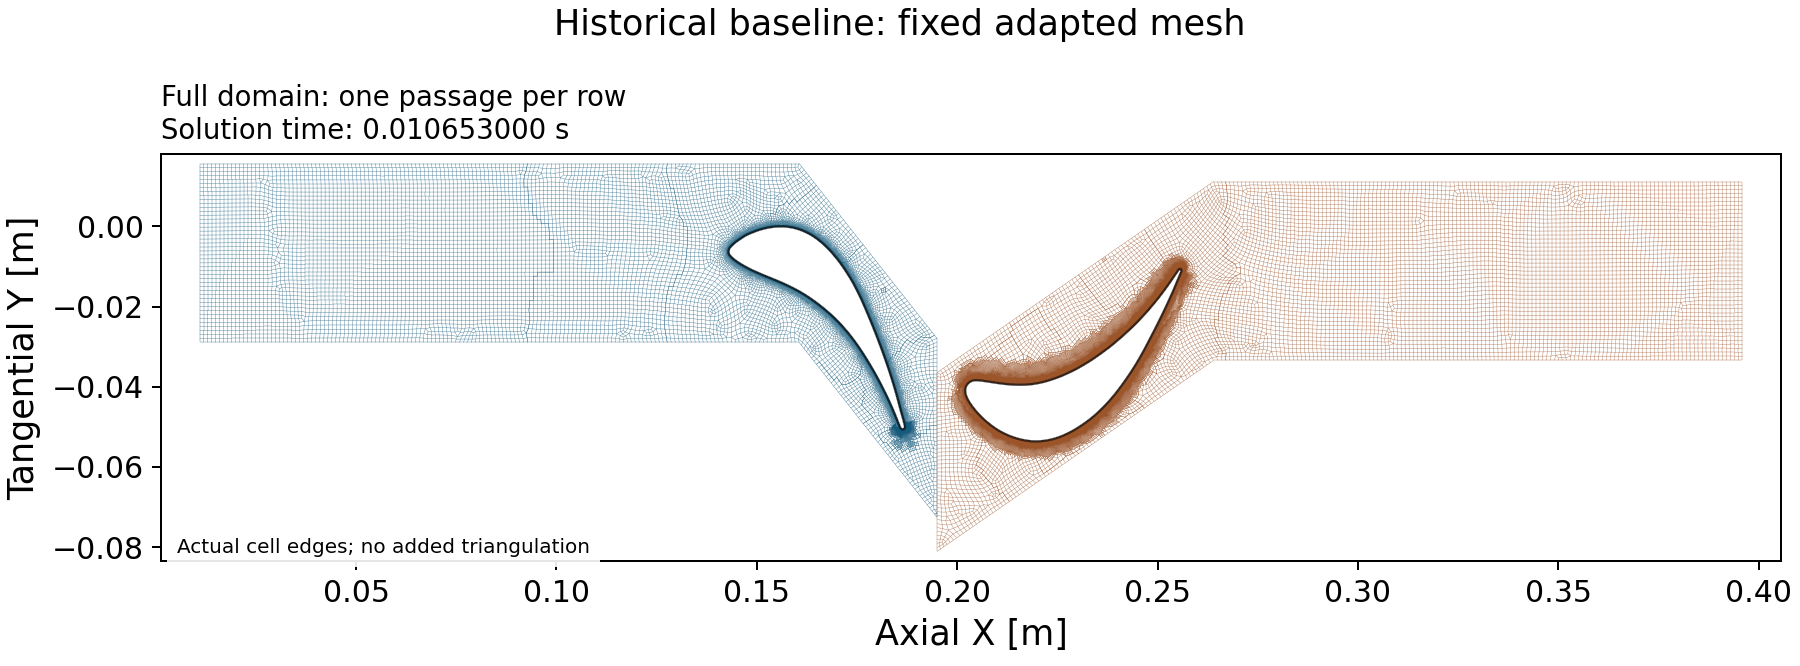
\includegraphics[width=\linewidth,height=0.42\textheight,keepaspectratio]{images/baseline_adapted_mesh.png}
\caption{Historical baseline mesh at t=0.010653 s. Actual polygon edges are shown; inactive AMR parents are excluded from active-cell statistics.}
\label{fig:1}
\end{figure}
\par
\subsection{Systematic mesh family and wall layers}
All three meshes use the same STEP and ANSYS Meshing procedure. Global sizing, curvature control, blade tangential spacing and first-layer height are refined together. The nominal inflation thickness remains 0.00094396216644 m. This is an anisotropic family; cell counts alone do not establish an asymptotic refinement sequence.\par

\par
\begin{table}[!htbp]
\centering
\caption{Systematic sizing and inflation controls}
\label{tab:5}
\small\renewcommand{\arraystretch}{1.16}
\begin{tabularx}{\linewidth}{@{}>{\raggedright\arraybackslash}X >{\raggedright\arraybackslash}X >{\raggedright\arraybackslash}X >{\raggedright\arraybackslash}X >{\raggedright\arraybackslash}X@{}}
\toprule
\textbf{Mesh} & \textbf{Global size [mm]} & \textbf{Blade spacing [mm]} & \textbf{First layer [micrometres]} & \textbf{Layers} \\
\midrule
M1 & 1.4 & 0.21 & 1 & 29 \\
M2 & 1 & 0.15 & 0.7142857 & 41 \\
M3 & 0.7142857 & 0.107142857 & 0.510204 & 57 \\
\bottomrule
\end{tabularx}
\end{table}
\par
\par
\begin{table}[!htbp]
\centering
\caption{Native active-cell counts and mesh-quality extrema}
\label{tab:6}
\small\renewcommand{\arraystretch}{1.16}
\begin{tabularx}{\linewidth}{@{}>{\raggedright\arraybackslash}X >{\raggedright\arraybackslash}X >{\raggedright\arraybackslash}X >{\raggedright\arraybackslash}X >{\raggedright\arraybackslash}X@{}}
\toprule
\textbf{Mesh} & \textbf{Active cells} & \textbf{Min orthogonal quality} & \textbf{Max aspect ratio} & \textbf{Max equiangle skewness} \\
\midrule
Historical adapted mesh & 289671 & 0.0263166 & 76.9229 & 0.6994222 \\
M1 & 54287 & 0.2461951 & 321.9638 & 0.7941735 \\
M2 & 104831 & 0.4701662 & 214.5706 & 0.7216187 \\
M3 & 196569 & 0.4183993 & 219.4238 & 0.7344144 \\
\bottomrule
\end{tabularx}
\end{table}
\par
The minimum orthogonal quality of the adapted mesh is only 0.0263166. The systematic meshes have positive cell volumes and minima of approximately 0.2462, 0.4702 and 0.4184. Quality is not monotonically improved by cell count. Their high aspect ratios occur in thin wall layers: all cells above aspect ratio 100 lie within approximately 11.36 micrometres of the corresponding blade, as checked against actual wall segments. This location does not replace a y+ or solution-quality check.\par

The direct systematic mesh exports are the authoritative meshes, stored locally as \path{inputs/meshes/M1_systematic.msh}, \path{M2_systematic.msh} and \path{M3_systematic.msh}. Historical Workbench FFF.msh caches contain 73167 cells and must not be substituted. Per-cell metrics, per-zone percentiles, threshold counts, extrema locations and native polygon-edge PNGs are retained with hashes in the technical archive. Selected quality tables and figures are supplied with the publication material. Raw-mesh screenshots and setup-verified screenshots are distinguished.\par

A bidirectional vertex-to-segment comparison checks actual blade-wall polylines at the baseline phase, without fitting a translation. The largest difference is 4.90 micrometres and includes curve tessellation differences. M2 discrepancies approach float32 coordinate resolution; these small values are not a claim of CAD accuracy at nanometre scale.\par

\par
\begin{table}[!htbp]
\centering
\caption{Geometry agreement from bidirectional blade-polyline matching}
\label{tab:7}
\small\renewcommand{\arraystretch}{1.16}
\begin{tabularx}{\linewidth}{@{}>{\raggedright\arraybackslash}X >{\raggedright\arraybackslash}X >{\raggedright\arraybackslash}X@{}}
\toprule
\textbf{Mesh} & \textbf{Blade} & \textbf{Maximum polyline difference [micrometres]} \\
\midrule
M1 & Stator & 4.897723 \\
M1 & Rotor & 2.590972 \\
M2 & Stator & 0.007679605 \\
M2 & Rotor & 0.01489774 \\
M3 & Stator & 2.627585 \\
M3 & Rotor & 1.50755 \\
\bottomrule
\end{tabularx}
\end{table}
\par
\par
\begin{figure}[!htbp]
\centering
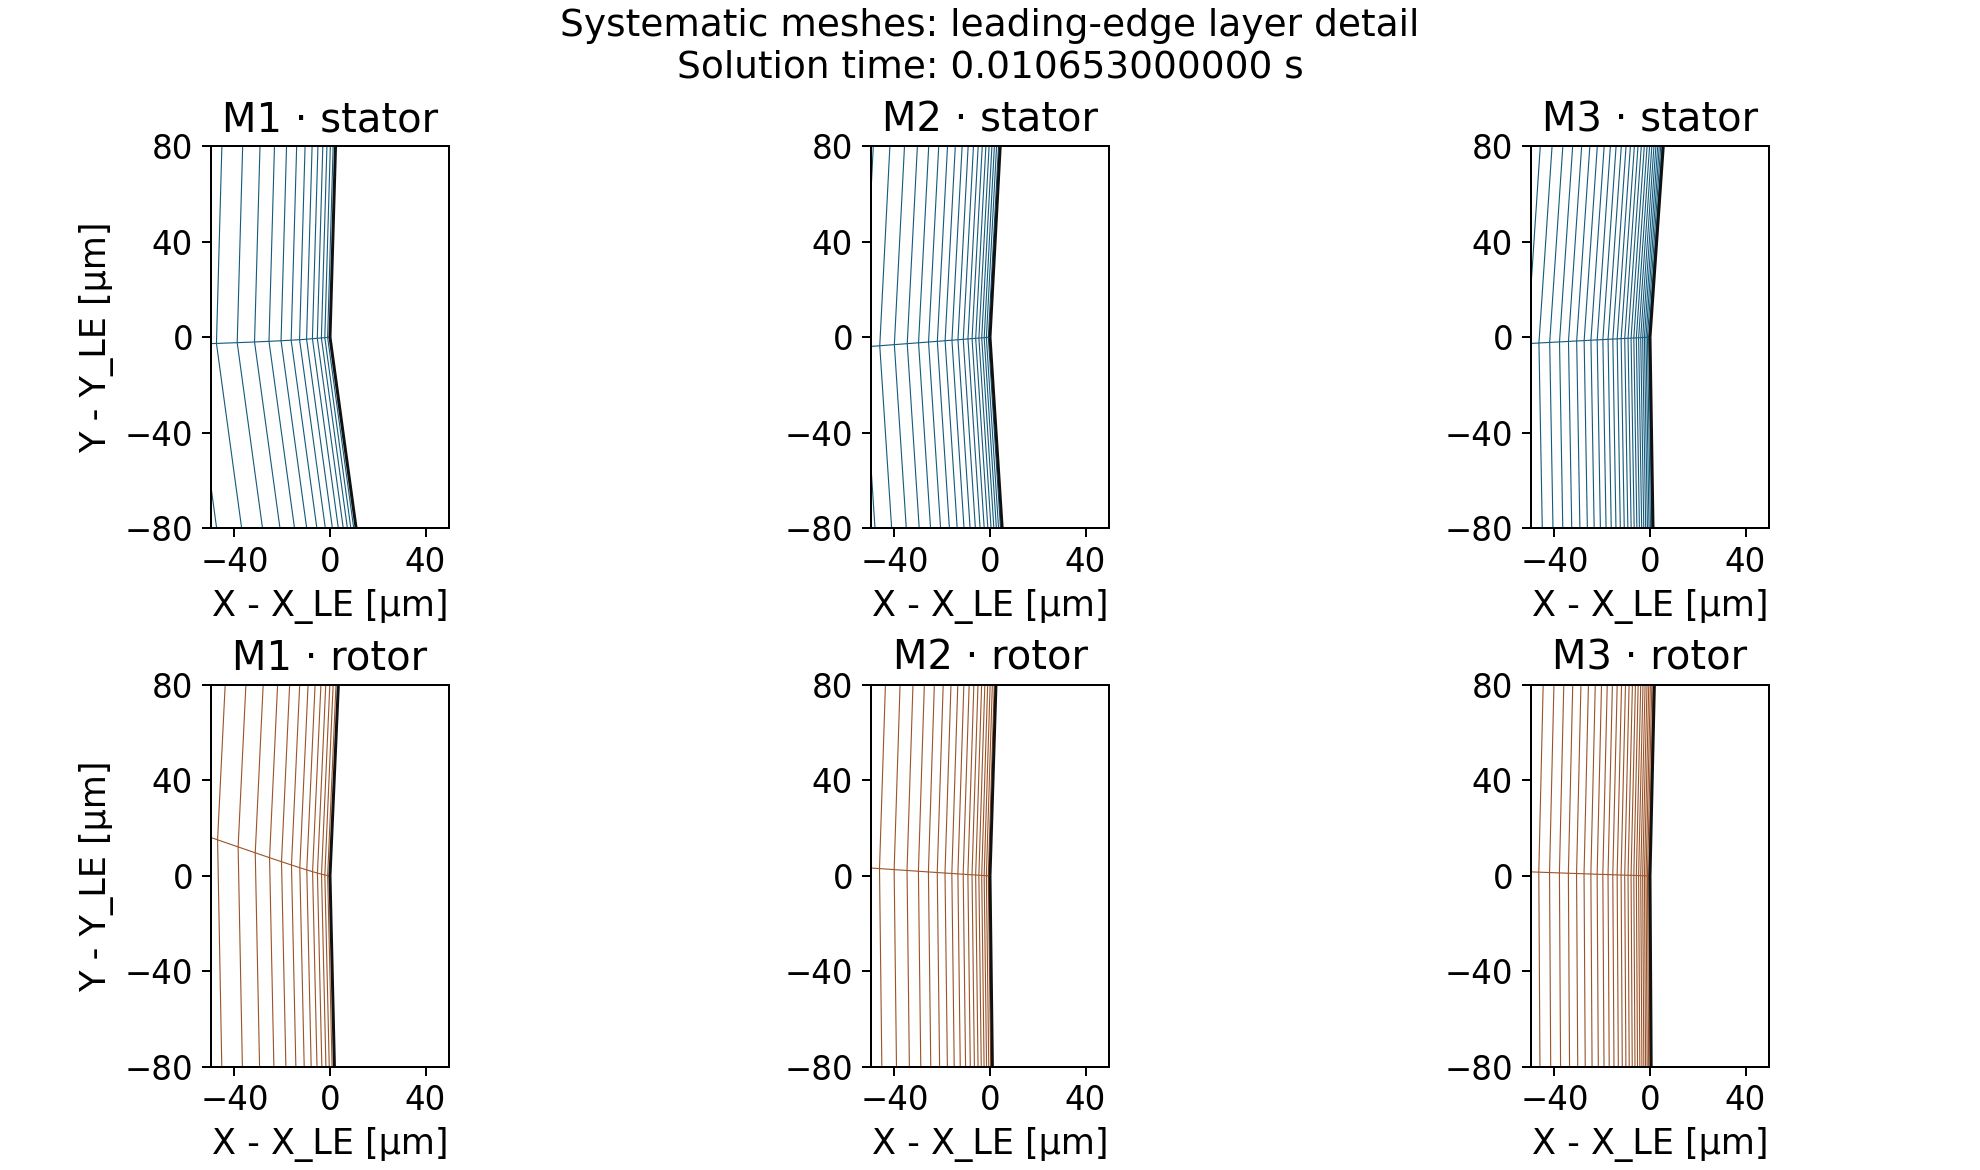
\includegraphics[width=\linewidth,height=0.42\textheight,keepaspectratio]{images/wall_layer_comparison.png}
\caption{Native leading-edge wall-layer detail for both rows. Coordinates are relative to the actual blade leading edge; no artificial triangular edges are added.}
\label{fig:2}
\end{figure}
\par
\par
\begin{figure}[!htbp]
\centering
\begin{subfigure}[t]{0.97\linewidth}\centering
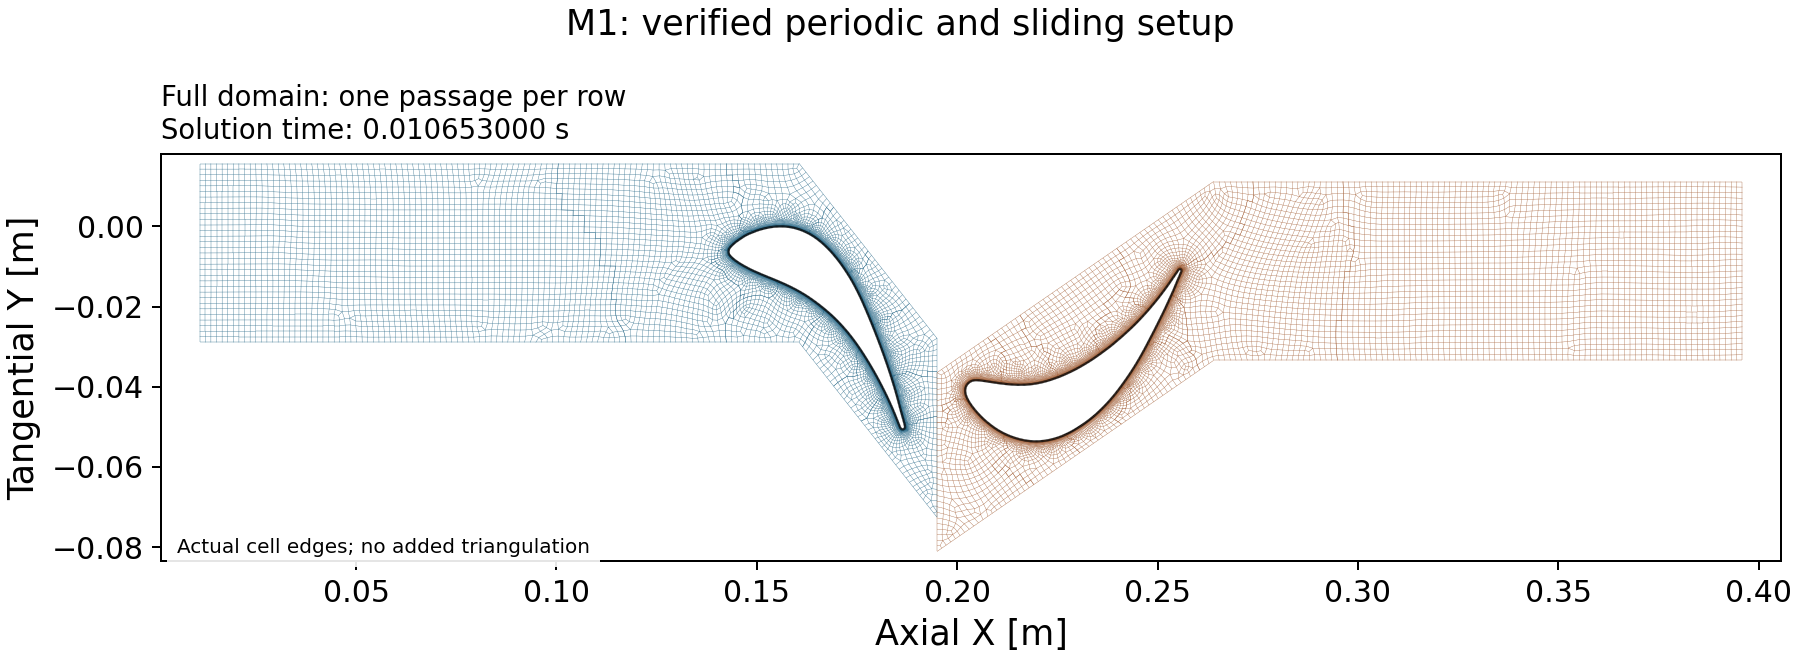
\includegraphics[width=\linewidth,height=0.235\textheight,keepaspectratio]{images/mesh_m1_domain.png}
\caption{M1, 54287 active cells}
\end{subfigure}
\par\vspace{0.65em}
\begin{subfigure}[t]{0.97\linewidth}\centering
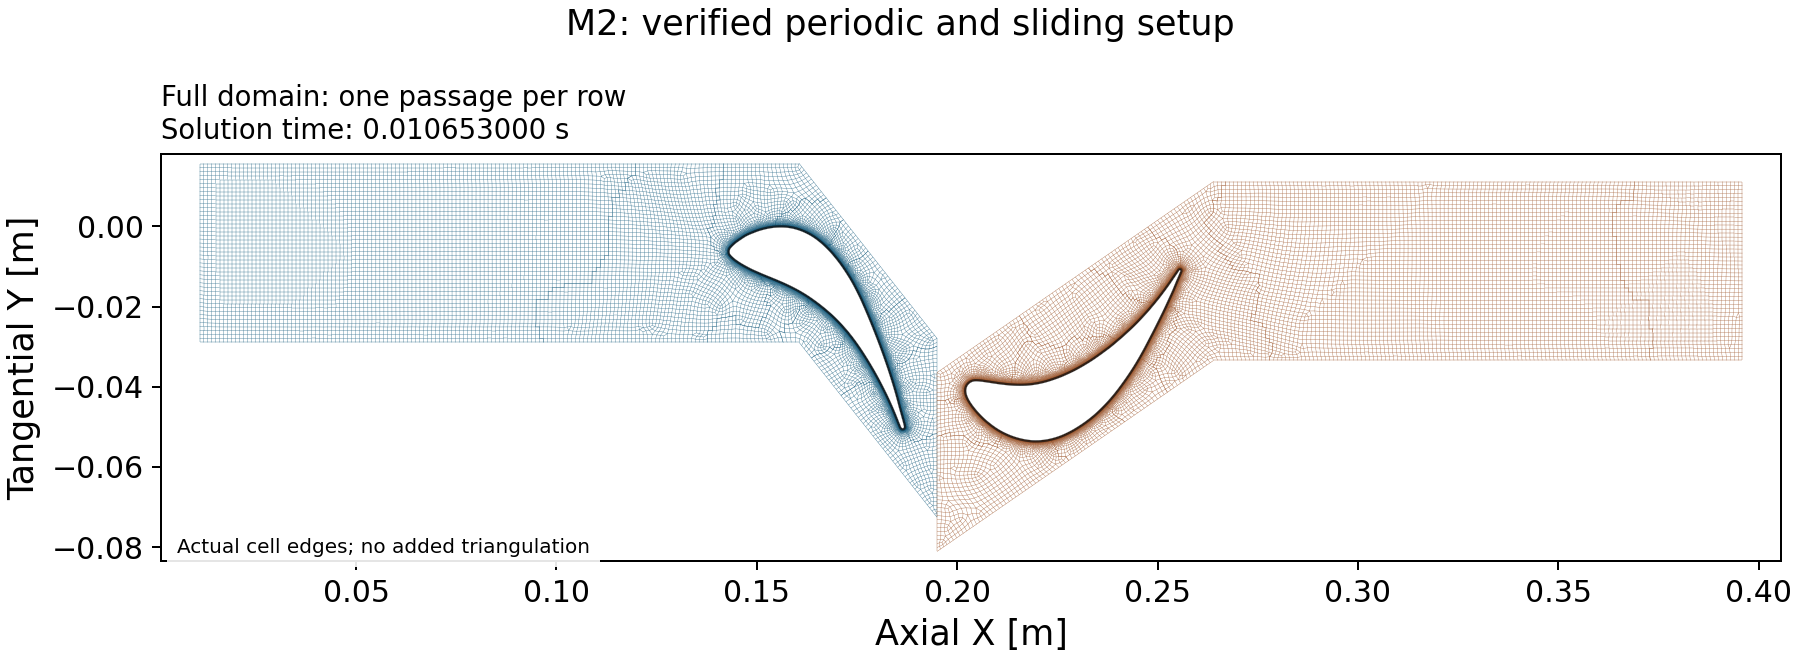
\includegraphics[width=\linewidth,height=0.235\textheight,keepaspectratio]{images/mesh_m2_domain.png}
\caption{M2, 104831 active cells}
\end{subfigure}
\par\vspace{0.65em}
\begin{subfigure}[t]{0.97\linewidth}\centering
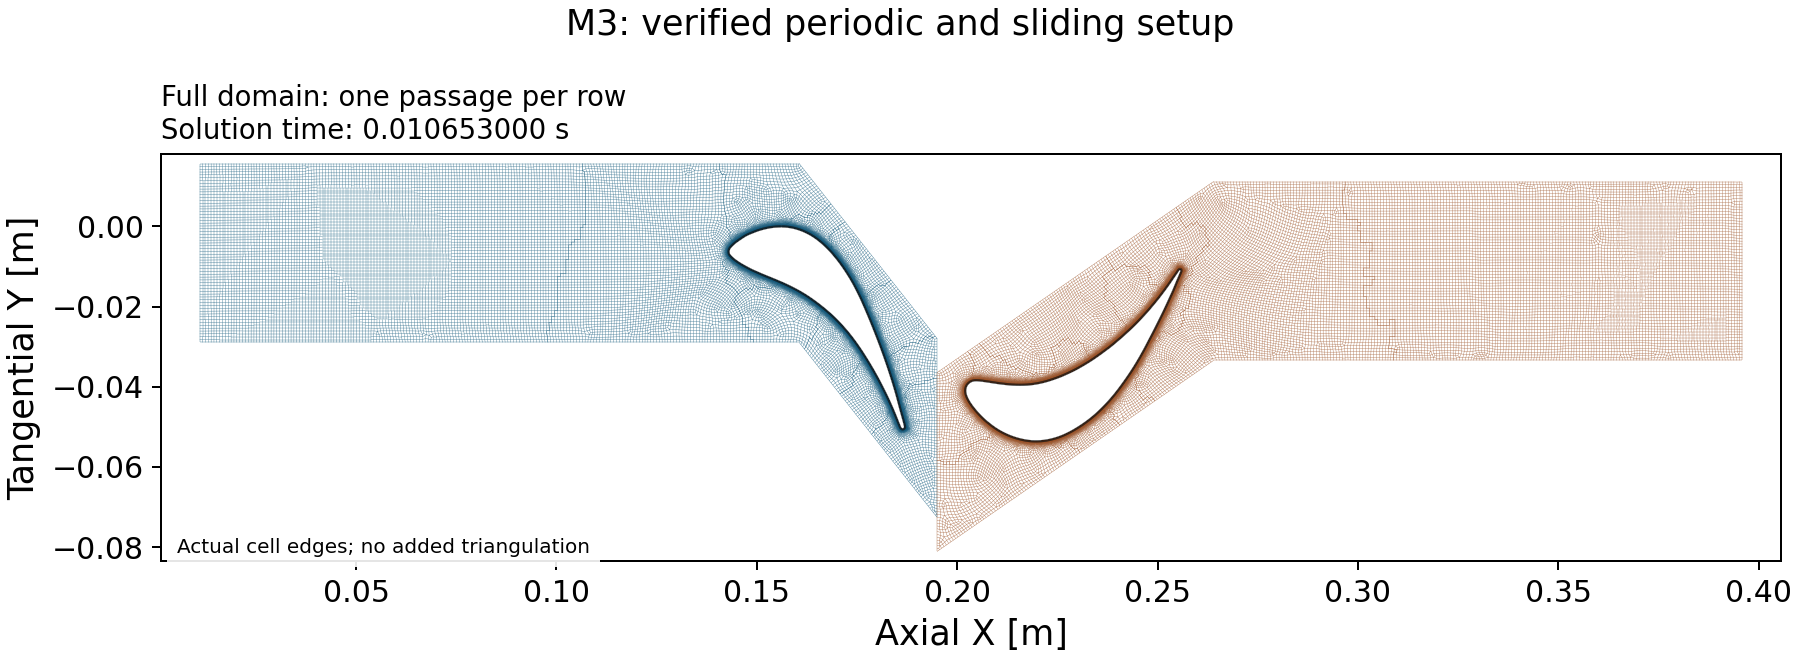
\includegraphics[width=\linewidth,height=0.235\textheight,keepaspectratio]{images/mesh_m3_domain.png}
\caption{M3, 196569 active cells}
\end{subfigure}
\par\vspace{0.65em}
\caption{Systematic family from the same geometry. These topology views were recorded at the inherited baseline phase during setup verification; original-position restoration for the accepted Hybrid runs is documented separately.}
\label{fig:3}
\end{figure}
\par
\par
\begin{figure}[!htbp]
\centering
\begin{subfigure}[t]{0.97\linewidth}\centering
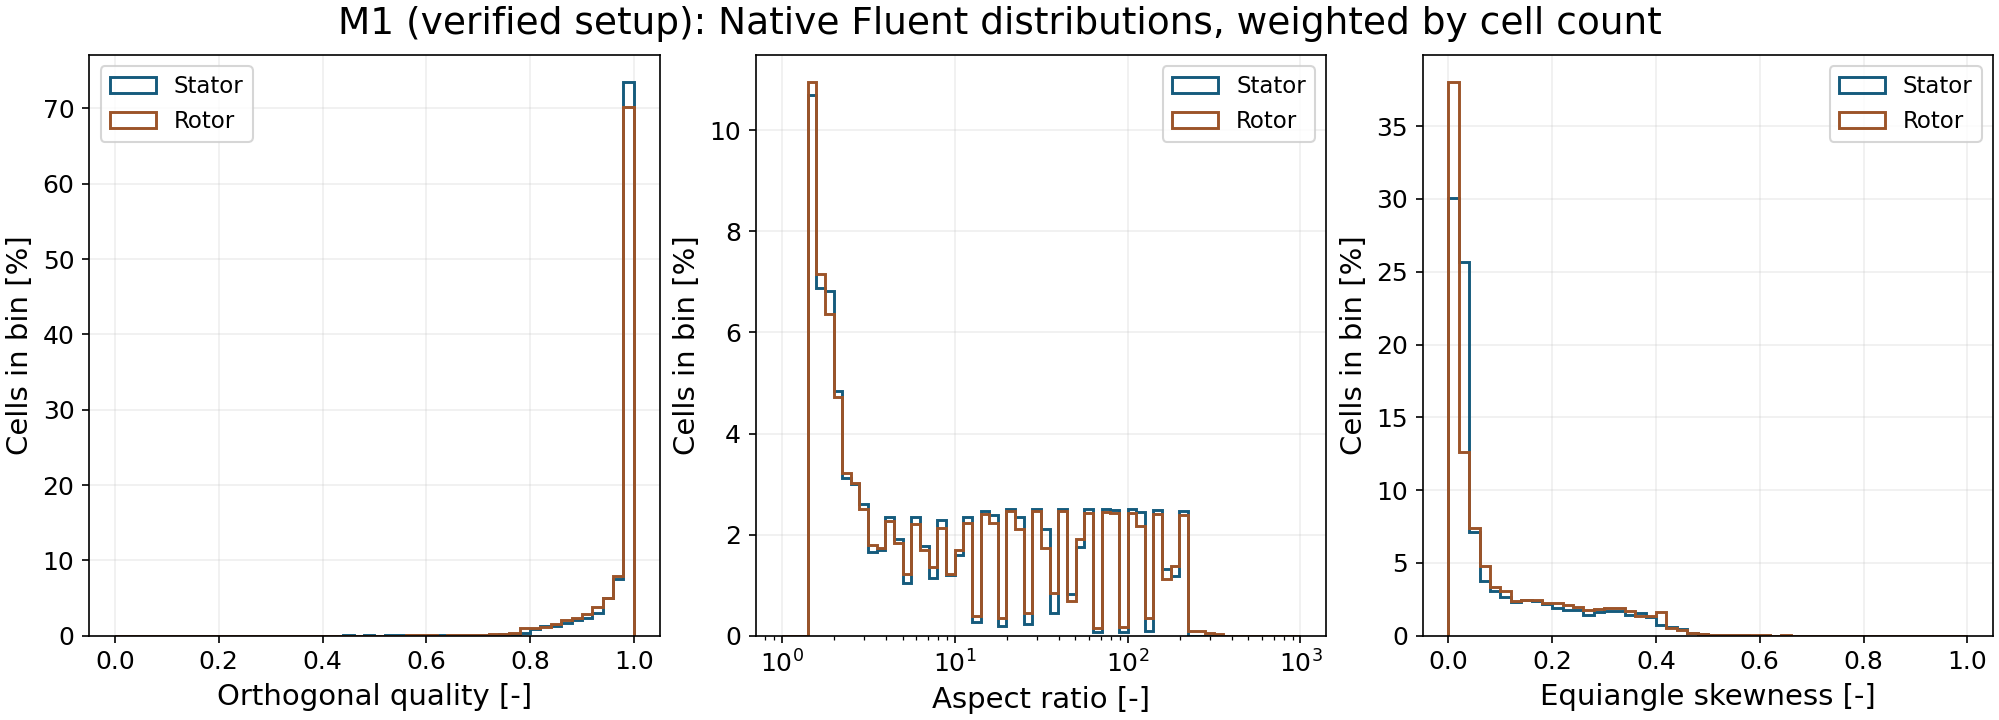
\includegraphics[width=\linewidth,height=0.235\textheight,keepaspectratio]{images/mesh_m1_quality_distributions.png}
\caption{M1}
\end{subfigure}
\par\vspace{0.65em}
\begin{subfigure}[t]{0.97\linewidth}\centering
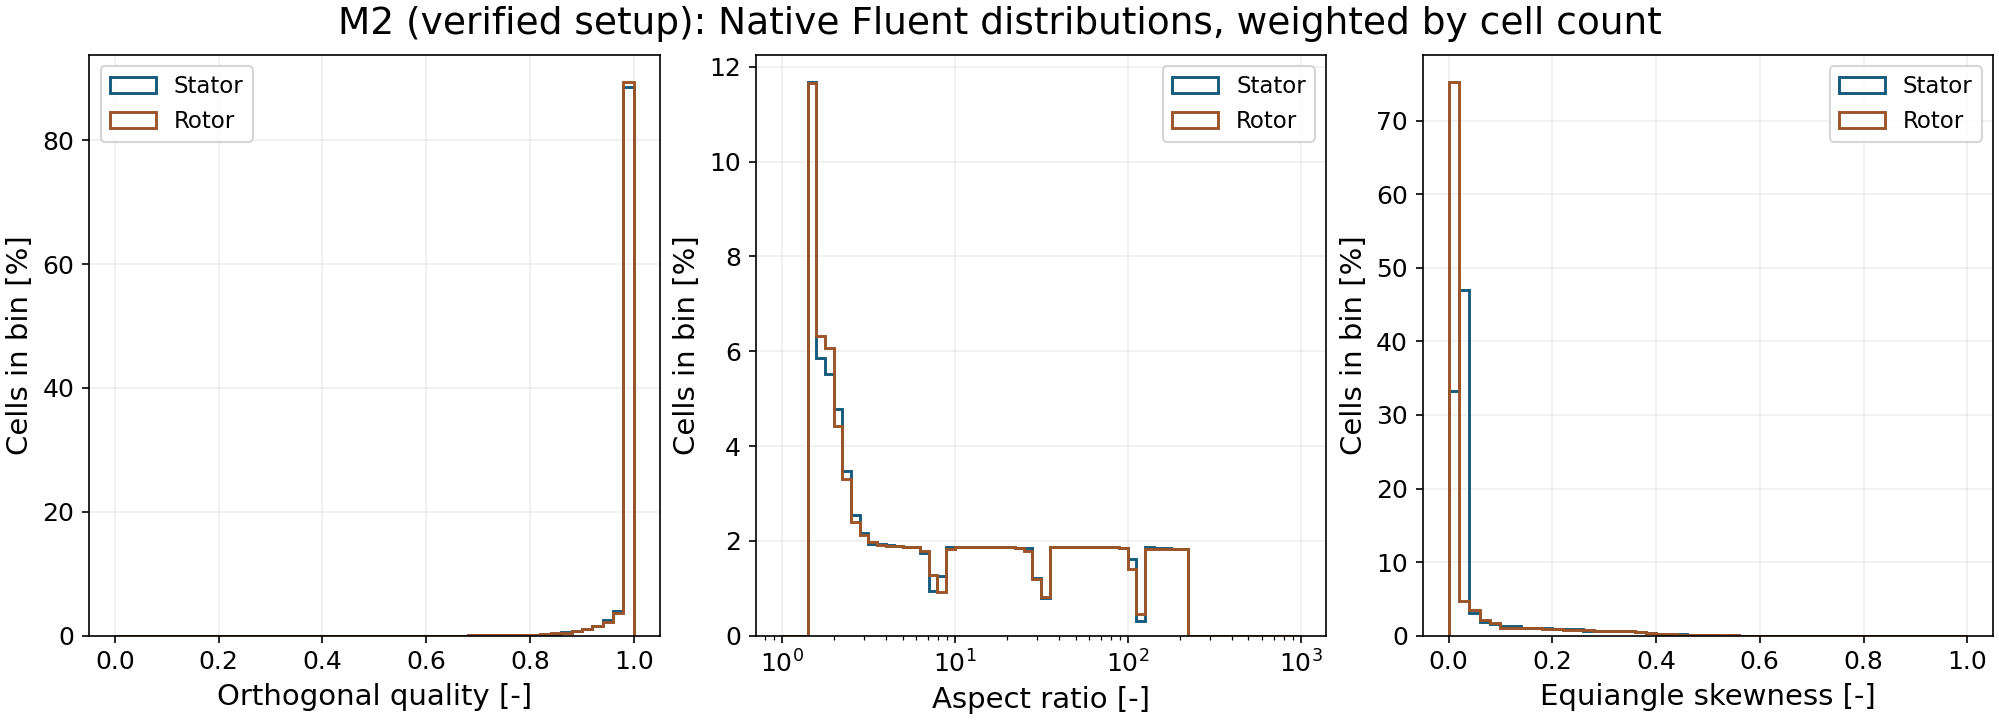
\includegraphics[width=\linewidth,height=0.235\textheight,keepaspectratio]{images/mesh_m2_quality_distributions.png}
\caption{M2}
\end{subfigure}
\par\vspace{0.65em}
\begin{subfigure}[t]{0.97\linewidth}\centering
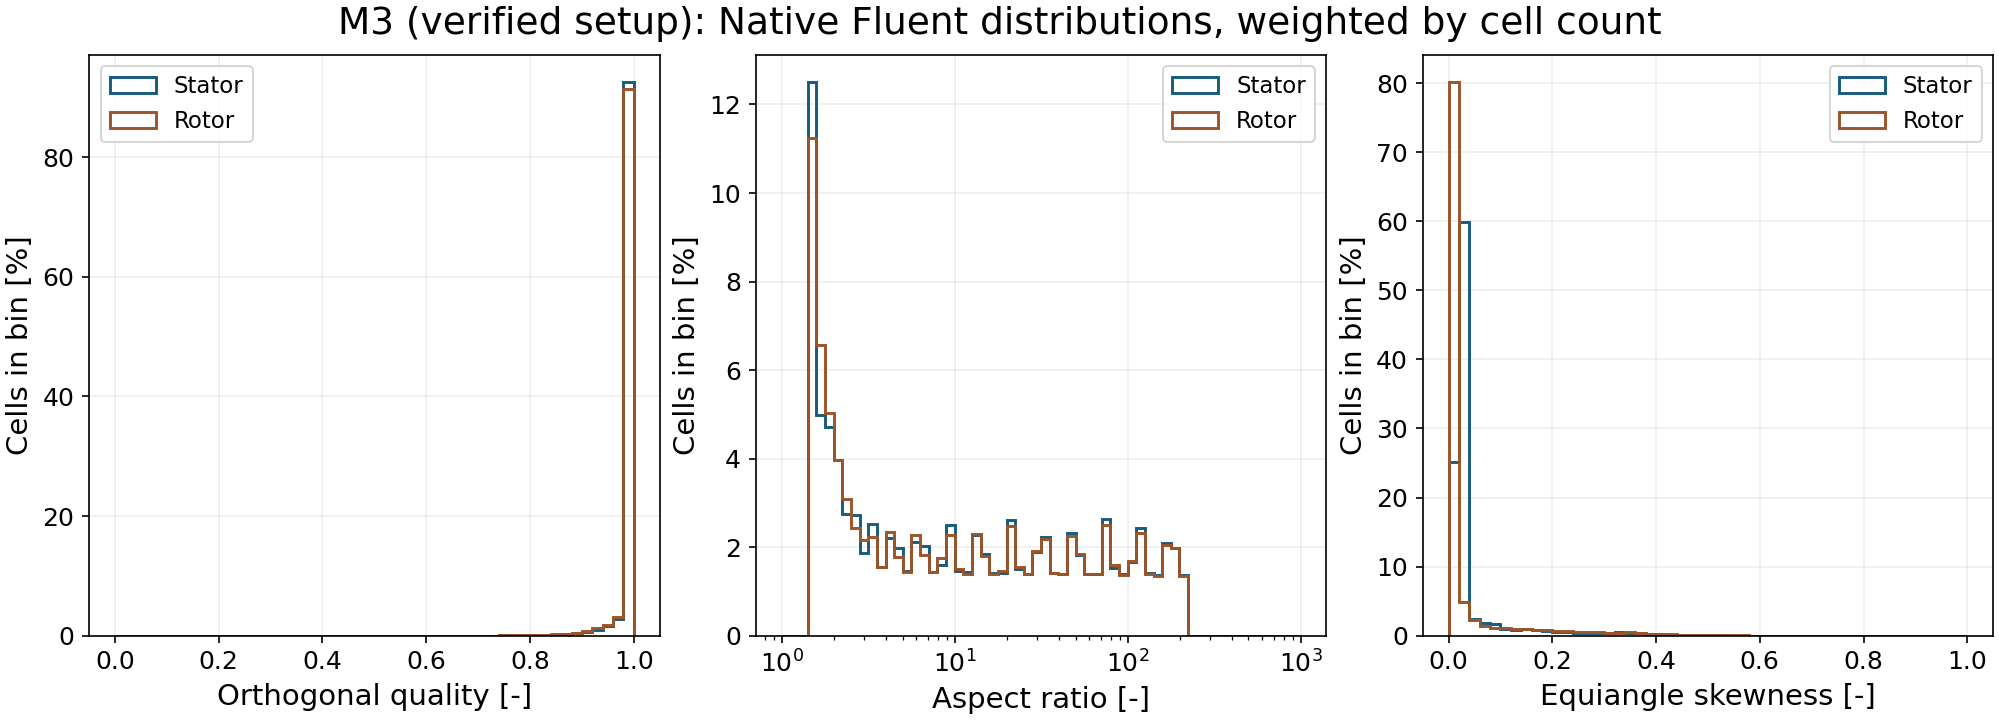
\includegraphics[width=\linewidth,height=0.235\textheight,keepaspectratio]{images/mesh_m3_quality_distributions.png}
\caption{M3}
\end{subfigure}
\par\vspace{0.65em}
\caption{Orthogonal quality, aspect ratio and skewness distributions. Each histogram is weighted by active cell count, not by cell volume.}
\label{fig:4}
\end{figure}
\par
\FloatBarrier
\section{Baseline integrity, initialization and native restart}
\subsection{Historical reference and dependencies}
The candidate final case/data pair was reopened together in an independent Fluent session. The verified native state is step 3551, physical time 0.010653 s and historical timestep 3e-6 s. Recomputed monitor values agree with the final historical samples. The baseline files remain unchanged.\par

\path{inputs/baseline/historical_baseline.cas.h5}: 9897196 bytes. SHA256: {\ttfamily\small c9f78c24\allowbreak{}b1a5263f\allowbreak{}655136f0\allowbreak{}c1a632ba\allowbreak{}4276c2ee\allowbreak{}c23a6e1b\allowbreak{}02622d72\allowbreak{}76378f7b}\par

\path{inputs/baseline/historical_baseline.dat.h5}: 73732083 bytes. SHA256: {\ttfamily\small 1038a1e4\allowbreak{}20ebfa1a\allowbreak{}47a87d00\allowbreak{}2627b207\allowbreak{}c05b8016\allowbreak{}d12ff650\allowbreak{}990773d7\allowbreak{}37710be1}\par

The local baseline inputs retain the original file contents under descriptive English names; the checksums above identify the historical pair independently of its filenames. The original Workbench .wbpj and its associated \_files directory are preserved together, without internal changes, in the private technical archive outside the repository. A separate portable Workbench archive includes the external STEP, was restored and reopened, and has ten checked internal Location references. The original absolute STEP reference was not changed.\par

The Fluent project index contained 132 absent historical references, corresponding to 66 case/data checkpoint pairs. The verified final restart did not require those checkpoints. Missing historical files were not recreated using data from different solution times. Native transcripts and SHA256 manifests were retained as provenance records.\par

\subsection{Common checkpoint and automated smoke test}
All adapted-mesh tests begin from the same verified checkpoint at t=0.010653 s and step 3551, without resetting time or reinitialising the solution. Output paths are redirected to independent run directories. The six-step smoke test advances dt=3e-6 s from 0.010653 to 0.010671 s, verifies approximately -0.0027 m of rotor translation, unchanged active cells, AMR disabled, monitor output, coherent saves, rereading and field rendering.\par

T400 resumed from a checkpoint after 120 steps at t=0.0107422751355 s, global step 3671. Five recomputed reports, including domain mass, matched exactly before further advance. Blade coordinates agreed with the checkpoint HDF5 within approximately 1.49e-8 m. Density, energy, turbulence variables, pressure, temperature and velocity retained their native first and second preceding time levels for second-order continuation. These time-history levels are distinct from the mesh identifiers M1 and M2. The restart occurred entirely within excluded settling.\par

Restart monitor segments have separate files and explicit time ranges. Coincident samples are merged only if both values and global steps agree. Fluent may add a restart-step suffix to a monitor filename; files are resolved through a unique native header and their actual paths/hashes are recorded. A fresh interpolation can omit the iteration-0 residual row; the residual parser checks the full 30-iteration countdown rather than subtracting the first printed row incorrectly.\par

\subsection{Original-position Hybrid initialization}
Preliminary interpolation and inherited-phase initialization trials were excluded from the systematic-mesh comparison. For the accepted campaign, the original rotor geometry was restored before Hybrid Initialization. This provided a consistent initial geometric phase on all three meshes.\par

For each active mesh, the rotor was restored to the actual geometry of the historical initial t=0 case before setting time and step to zero and applying Fluent Hybrid Initialization. The M3 restoration included a measured Y correction of -0.000900000333786 m. No historical solution data or interpolation field was loaded for initialization. A separate six-step smoke test verified positive fields, motion and restart; the main calculation reread the fresh initialized pair. All active calculations use 24 MPI ranks, dt=T/400=7.439594625e-7 s, 30 actual inner iterations per step and disabled automatic adaptation. Restarts preserve time, rotor geometry and BDF2 history.\par

\par
\begin{figure}[!htbp]
\centering
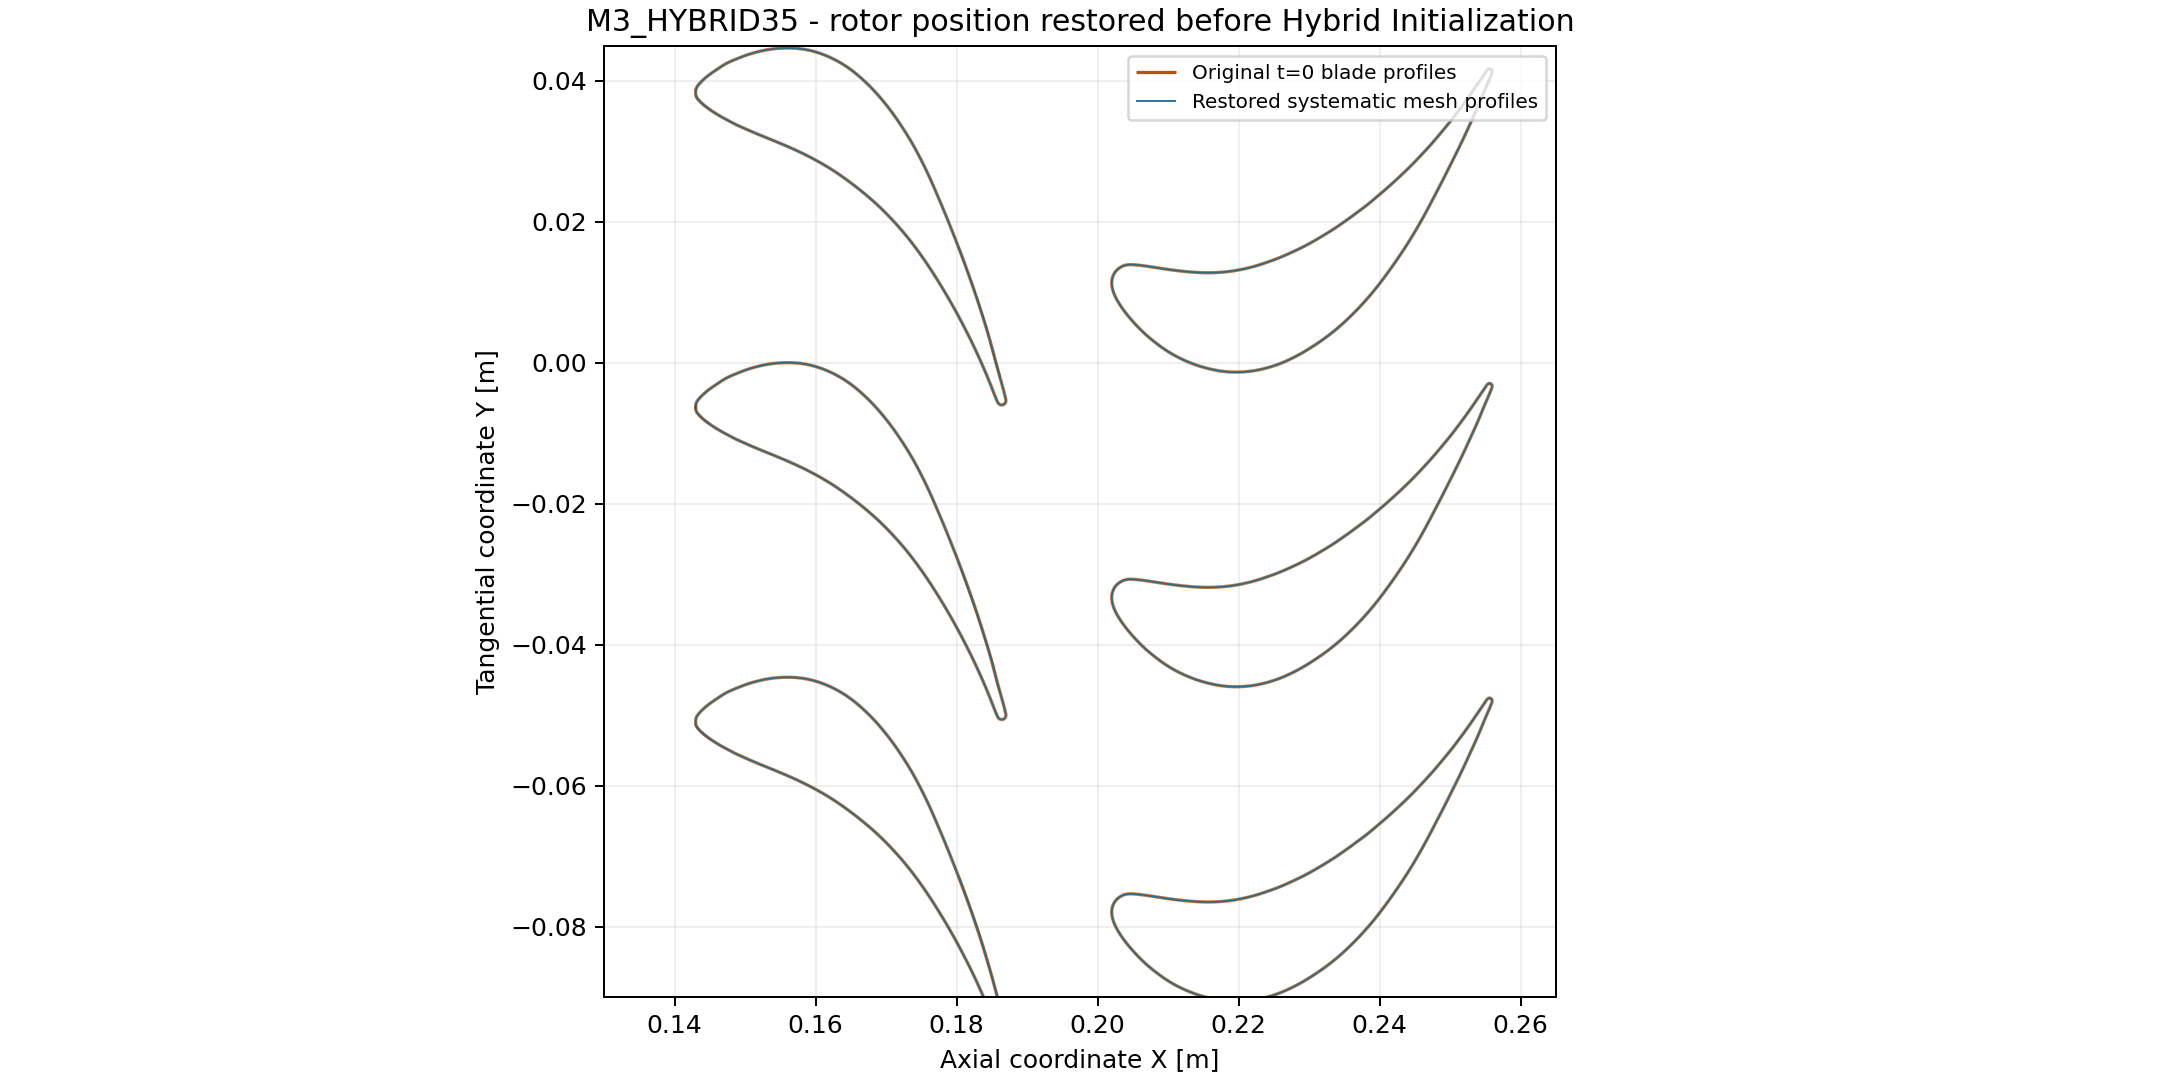
\includegraphics[width=\linewidth,height=0.42\textheight,keepaspectratio]{images/initial_rotor_position.png}
\caption{M3 rotor restoration against the actual historical t=0 geometry before Hybrid Initialization. Resetting time without this geometry check would define a different initial position.}
\label{fig:5}
\end{figure}
\par
\FloatBarrier
\section{Numerical verification}
\subsection{Definitions, statistical windows and recurrence criteria}
Three complete blade-passing cycles are compared at the same rotor phase. Cycle means use trapezoidal integration of the native full-precision clock; cycle peak-to-peak amplitudes are calculated before averaging. Phase profiles use 401 points per cycle. The primary quantities are\par

\begin{align}
\overline{q}&=\frac{1}{3T}\int_{t_a}^{t_a+3T}q(t)\,\mathrm{d}t, &
\overline{A}&=\frac{1}{3}\sum_{k=1}^{3}\left(\max_{t\in I_k}q(t)-\min_{t\in I_k}q(t)\right).
\end{align}
\par
\begin{table}[!htbp]
\centering
\caption{Unchanged diagnostic limits. They are not experimental-accuracy or grid-independence tolerances.}
\label{tab:8}
\small\renewcommand{\arraystretch}{1.16}
\begin{tabularx}{\linewidth}{@{}>{\raggedright\arraybackslash}X >{\raggedright\arraybackslash}X >{\raggedright\arraybackslash}X@{}}
\toprule
\textbf{Diagnostic} & \textbf{Operational limit} & \textbf{Meaning} \\
\midrule
Consecutive cycle means & 0.5\% & Relative to the later cycle mean \\
Consecutive amplitudes & 5\% & Relative to the later cycle amplitude \\
Phase-profile RMS & 10\% of amplitude & Cycle-to-cycle recurrence \\
Mean inlet/outlet imbalance & 0.5\% & Boundary-flux check \\
Integrated defect with storage & 0.01\% & Compressible mass conservation \\
Phase-matched nodal field RMS & 0.5\% & Operational field recurrence; not volume weighted \\
\bottomrule
\end{tabularx}
\end{table}
\par
\par
\begin{table}[!htbp]
\centering
\caption{Accepted original-position Hybrid campaign at closure. All runs use T/400, 30 inner iterations and 24 MPI processes.}
\label{tab:9}
\small\renewcommand{\arraystretch}{1.16}
\begin{tabularx}{\linewidth}{@{}>{\raggedright\arraybackslash}X >{\raggedright\arraybackslash}X >{\raggedright\arraybackslash}X >{\raggedright\arraybackslash}X >{\raggedright\arraybackslash}X@{}}
\toprule
\textbf{Mesh} & \textbf{Active cells} & \textbf{Periods} & \textbf{Statistics cycles} & \textbf{Monitor recurrence} \\
\midrule
M1 & 54,287 & 35 & 33-35 & Passed recorded limits \\
M2 & 104,831 & 40 & 38-40 & Inlet amplitude: 7.7537\% > 5\% \\
M3 & 196,569 & 35 & 33-35 & Force amplitude: 7.0685\% > 5\% \\
\bottomrule
\end{tabularx}
\end{table}
\par
M3 reached 14000 accepted steps and t=0.010415432475 s. Its force amplitudes in cycles 33, 34 and 35 are 199.4099756, 186.2452157 and 185.6334933 N. The last change is only 0.329532\%, but the previous change is 7.068509\%; the required three-cycle check therefore fails. M2 and M3 remain unconfirmed under the original limits. Failed graphics-replay frames and an earlier unsaved monitor tail are excluded from the accepted main histories.\par

\par
\begin{figure}[!htbp]
\centering
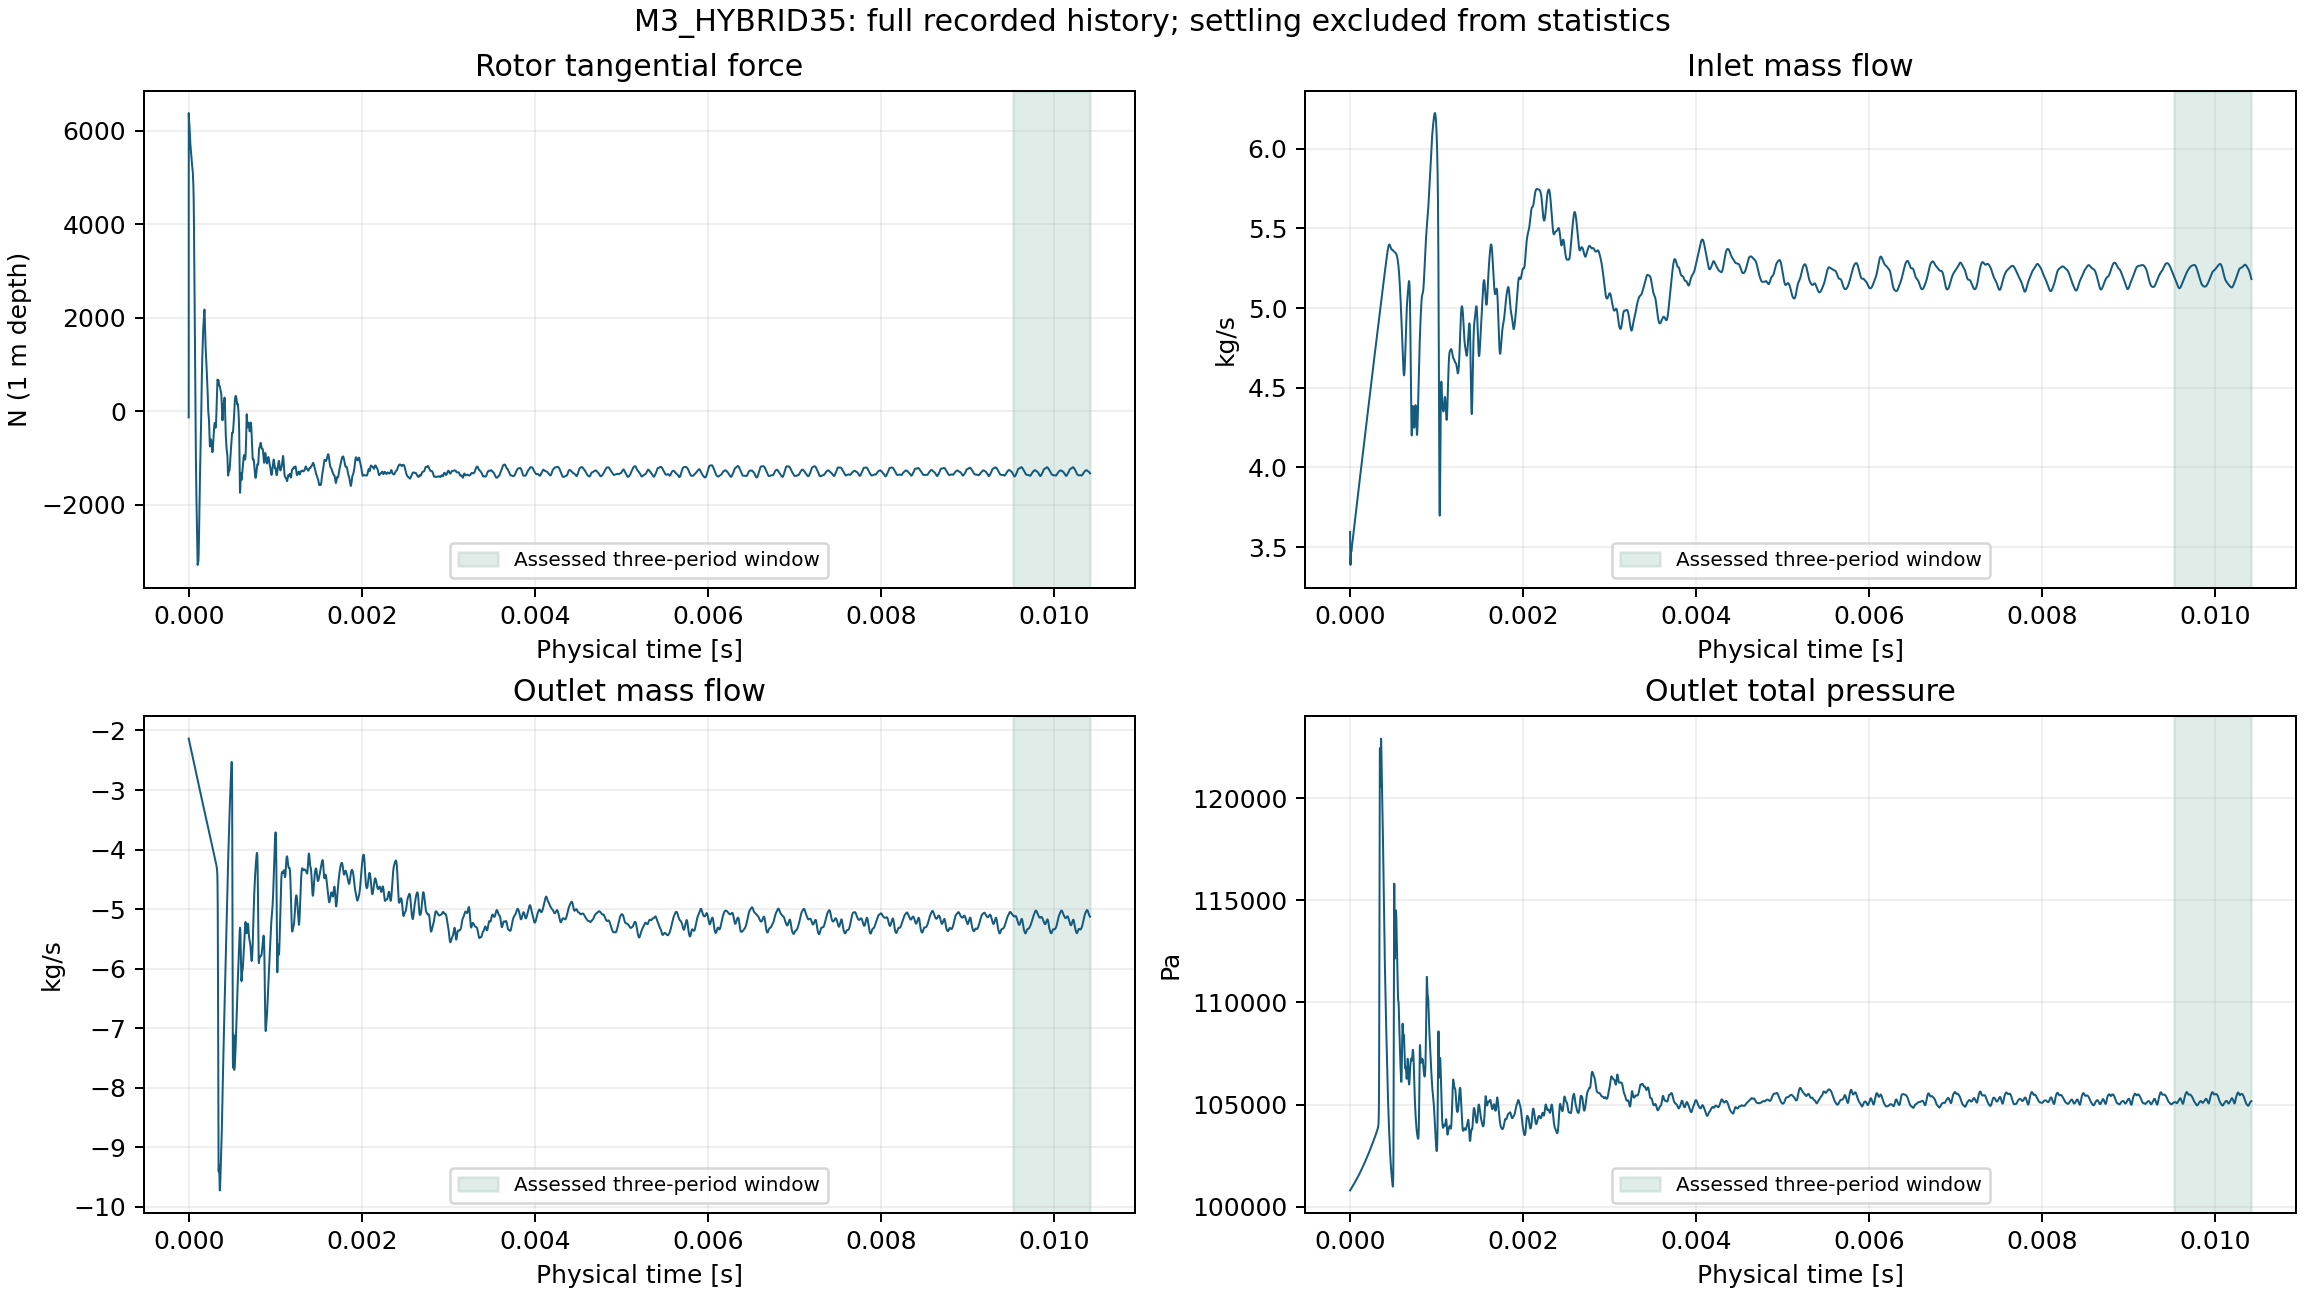
\includegraphics[width=\linewidth,height=0.42\textheight,keepaspectratio]{images/m3_monitor_time_histories.png}
\caption{M3 fresh-Hybrid monitor history to 35 periods. The shaded interval is the assessed three-cycle window; the initial transient is not part of its statistics.}
\label{fig:6}
\end{figure}
\par
\par
\begin{figure}[!htbp]
\centering
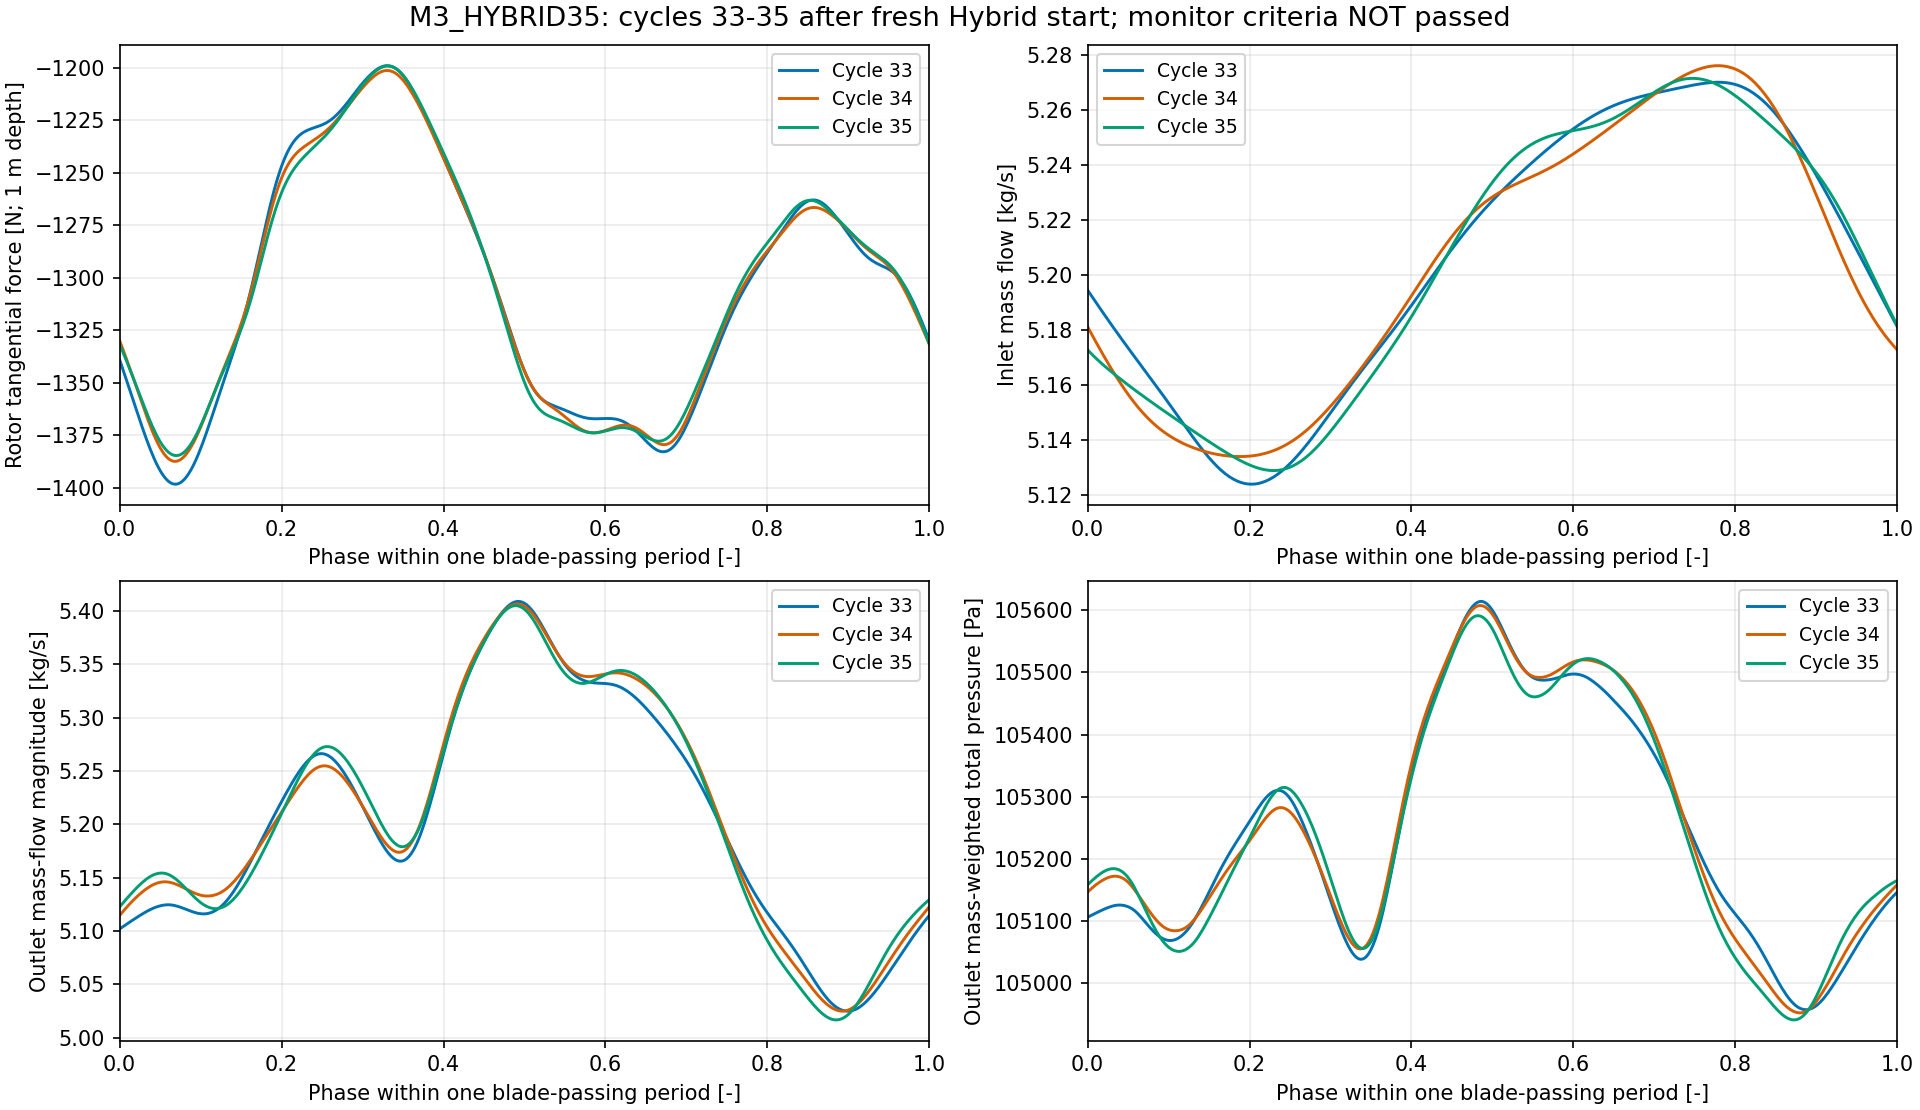
\includegraphics[width=\linewidth,height=0.42\textheight,keepaspectratio]{images/m3_cycle_recurrence.png}
\caption{M3 cycle recurrence at common rotor phase. Means are stable, while the force-amplitude test still fails for cycles 33 to 34.}
\label{fig:7}
\end{figure}
\par
\subsection{Compressible conservation and native field recurrence}
The correct signed mass balance is dM/dt = mass flow at inlet + mass flow at outlet. Integrating the fluxes over a cycle must reproduce the change of mass stored in the domain. A nonzero instantaneous inlet/outlet difference can be physical storage; conservation and periodic recurrence must be checked separately.\par

The reported integrated mass defect is normalised by the mass transported through the inlet over the same cycle:
\begin{equation}
\epsilon_M=100\frac{\left|\int_{t_a}^{t_b}(\dot m_{\mathrm{in}}+\dot m_{\mathrm{out}})\,\mathrm{d}t-[M(t_b)-M(t_a)]\right|}{\int_{t_a}^{t_b}|\dot m_{\mathrm{in}}|\,\mathrm{d}t}.
\end{equation}
Trapezoidal integration is used for this cycle-integrated diagnostic. The instantaneous BDF2 defect is evaluated separately using the native constant timestep.\par

\par
\begin{table}[!htbp]
\centering
\caption{Recorded conservation, field-recurrence and wall-resolution diagnostics. Passing these checks does not replace the failed monitor-amplitude test.}
\label{tab:10}
\small\renewcommand{\arraystretch}{1.16}
\begin{tabularx}{\linewidth}{@{}>{\raggedright\arraybackslash}X >{\raggedright\arraybackslash}X >{\raggedright\arraybackslash}X >{\raggedright\arraybackslash}X@{}}
\toprule
\textbf{Mesh} & \textbf{Max integrated mass defect [\%]} & \textbf{Max nodal recurrence RMS [\%]} & \textbf{Stator / rotor sampled max y+} \\
\midrule
M1 & 1.02818e-05 & 0.133355 & 0.5837 / 0.5240 \\
M2 & 1.1913e-05 & 0.325564 & 0.4625 / 0.3745 \\
M3 & 1.55443e-05 & 0.237437 & 0.3082 / 0.2682 \\
\bottomrule
\end{tabularx}
\end{table}
\par
For matched unique export coordinates, the relative nodal recurrence norm compares an earlier field $q_A$ with the field $q_B$ one period later:
\begin{equation}
\epsilon_q=100\frac{\sqrt{N^{-1}\sum_{i=1}^{N}(q_{B,i}-q_{A,i})^2}}{\sqrt{N^{-1}\sum_{i=1}^{N}q_{B,i}^2}}.
\end{equation}
The denominator is the RMS of the later absolute field, without subtracting its mean; the norm is evaluated separately for each field and fluid zone. Coincident export coordinates can carry differing nodal values. In those cases the assessment uses the largest possible difference at each coordinate and a lower bound for the reference-field RMS to obtain a conservative upper bound over every value selection. No values are averaged or excluded, and the 0.5\% limit is unchanged. Identical duplicate values reproduce the unique-coordinate norm above. This exported-node norm is not volume weighted and is not a spatial-discretisation error estimate.\par

\par
\begin{figure}[!htbp]
\centering
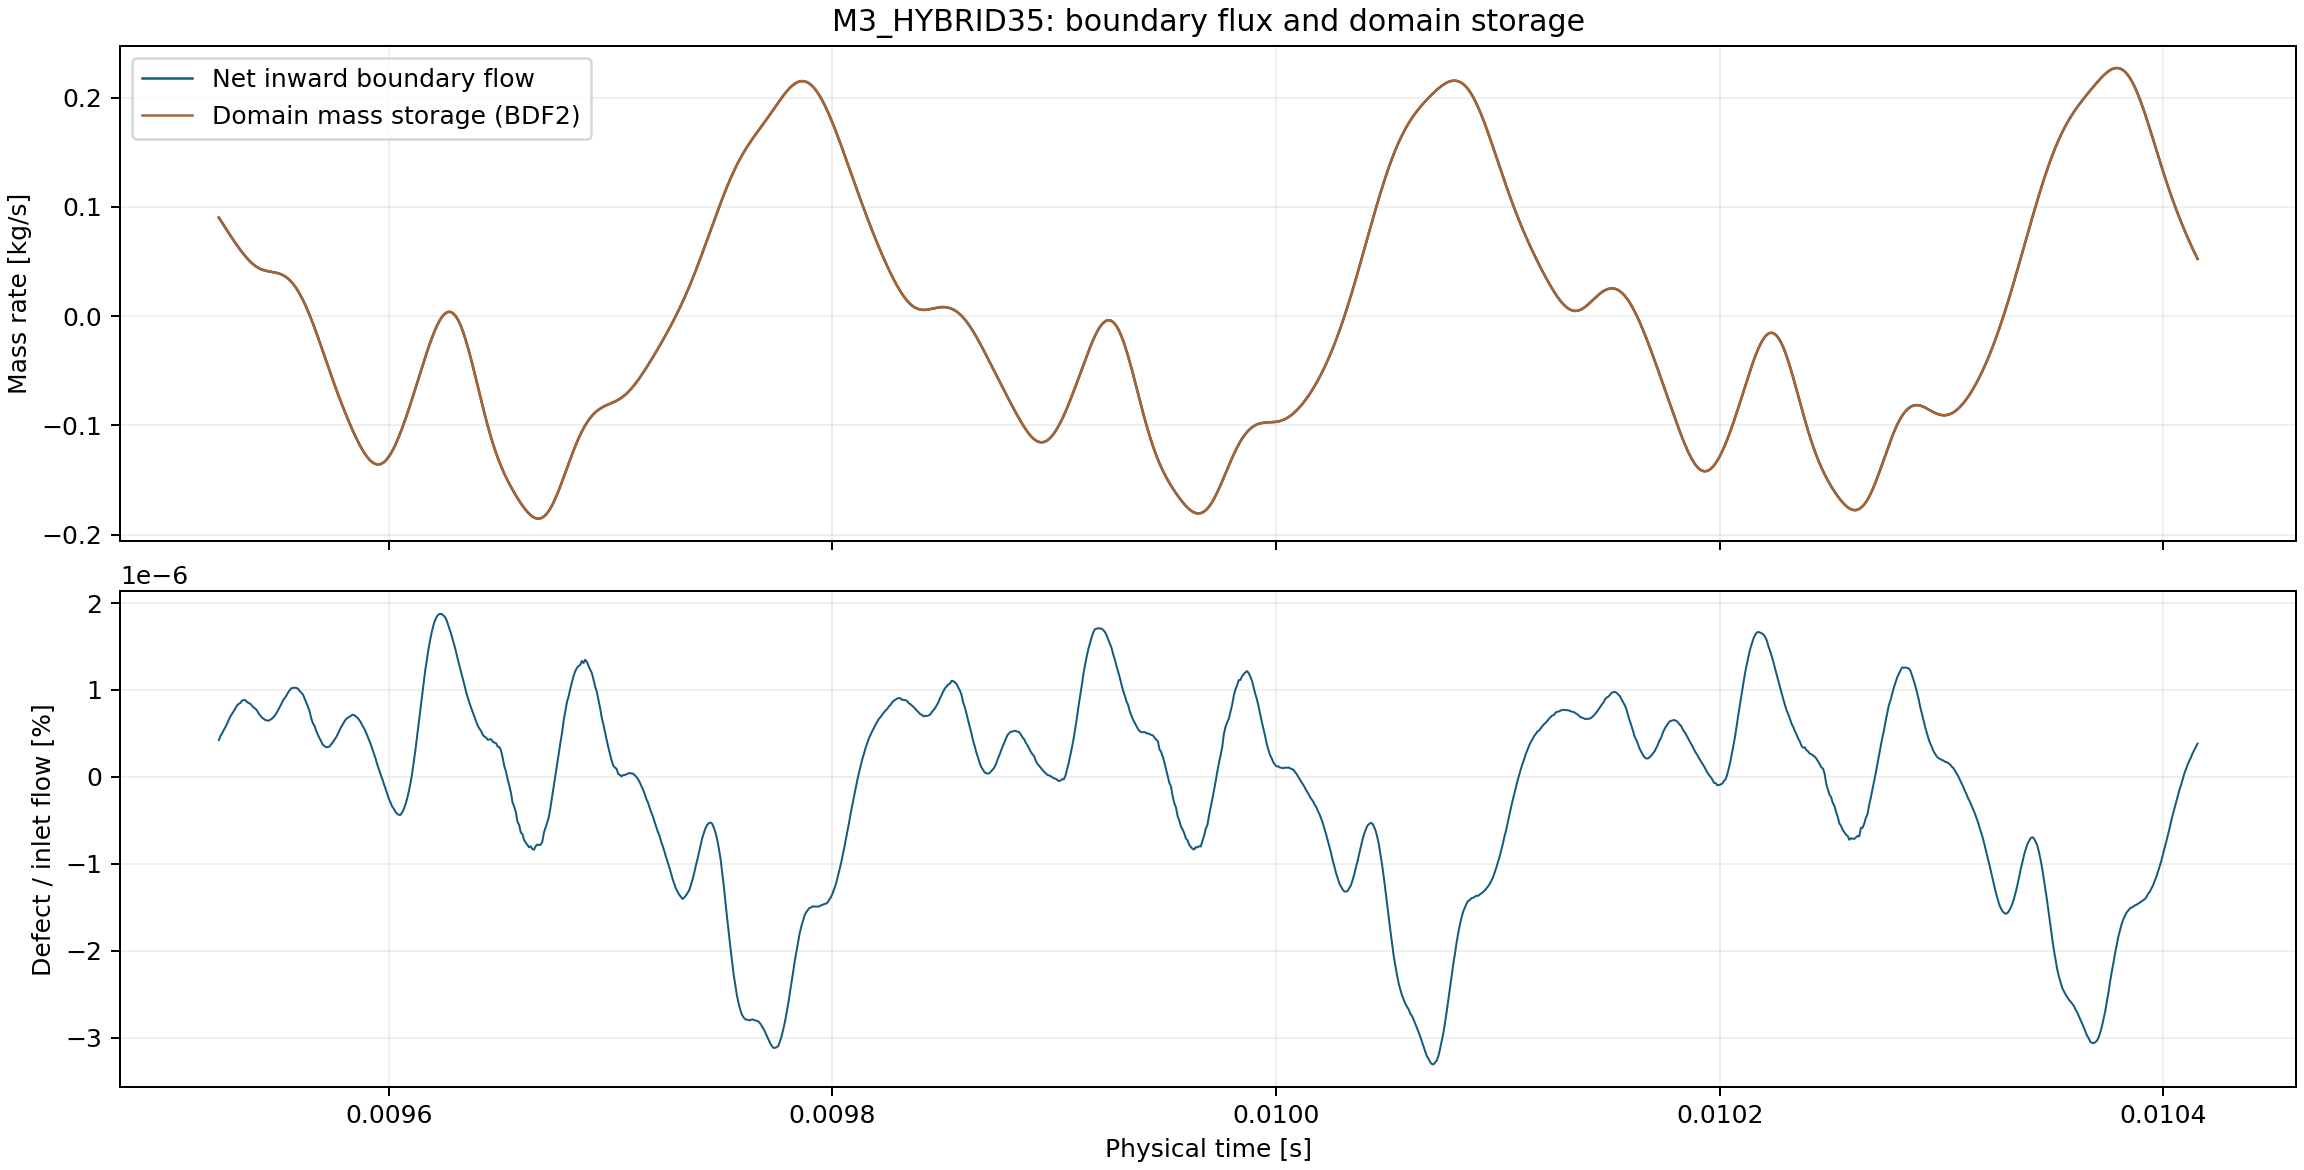
\includegraphics[width=\linewidth,height=0.42\textheight,keepaspectratio]{images/m3_mass_conservation.png}
\caption{Native boundary flux and BDF2 domain-mass storage over the final M3 window. The small difference is the conservative defect, not the full boundary-flux imbalance.}
\label{fig:8}
\end{figure}
\par
\subsection{Inner-iteration sensitivity on the adapted mesh}
ITER30 and ITER60 use identical initial fields, mesh, timestep and phase-aligned statistical windows. Residual-based early stopping is disabled to perform exactly 30 or 60 inner iterations per step. ITER30 initially used 8 processes for its first 240 settling steps; it then resumed at 24 processes. Its entire statistical window, ITER60 and all subsequent tests use 24 MPI ranks. Rank count is verified; physical-core affinity is not claimed.\par

\par
\begin{table}[!htbp]
\centering
\caption{ITER30/ITER60 comparison on identical initial fields and phase windows}
\label{tab:11}
\small\renewcommand{\arraystretch}{1.16}
\begin{tabularx}{\linewidth}{@{}>{\raggedright\arraybackslash}X >{\raggedright\arraybackslash}X >{\raggedright\arraybackslash}X >{\raggedright\arraybackslash}X >{\raggedright\arraybackslash}X@{}}
\toprule
\textbf{Comparison} & \textbf{Monitor} & \textbf{Mean diff. [\%]} & \textbf{Amplitude diff. [\%]} & \textbf{Phase RMS / amp. [\%]} \\
\midrule
ITER30/ITER60 & Rotor tangential force & 0.008112165 & 1.100442 & 0.6270705 \\
ITER30/ITER60 & Inlet mass flow & 0.000778778 & 1.402773 & 0.6348632 \\
ITER30/ITER60 & Outlet mass flow & 0.003901606 & 0.669901 & 0.4889742 \\
ITER30/ITER60 & Outlet mass-flow-weighted total pressure & 0.0002717684 & 0.6225031 & 0.5274144 \\
\bottomrule
\end{tabularx}
\end{table}
\par
The largest mean difference is approximately 0.00812\%, amplitude difference 1.403\%, and phase RMS 0.635\% of amplitude. These satisfy the proposed 0.1\% / 2\% / 2\% operational comparison limits, supporting an initial choice of 30 inner iterations. They remain uncertainty scales when interpreting smaller timestep or mesh differences. Nodal same-phase field norms are not volume-weighted error estimates.\par

\subsection{Temporal sensitivity on the adapted mesh}
\par
\begin{table}[!htbp]
\centering
\caption{Timestep-study settings and complete-cycle statistical windows}
\label{tab:12}
\small\renewcommand{\arraystretch}{1.16}
\begin{tabularx}{\linewidth}{@{}>{\raggedright\arraybackslash}X >{\raggedright\arraybackslash}X >{\raggedright\arraybackslash}X >{\raggedright\arraybackslash}X >{\raggedright\arraybackslash}X@{}}
\toprule
\textbf{Run} & \textbf{Timestep [s]} & \textbf{Steps} & \textbf{Excluded periods} & \textbf{Statistics [s]} \\
\midrule
T100 & 2.975838e-06 & 600 & 3 & 0.011545751355 - 0.012438502710 \\
T200 & 1.487919e-06 & 1200 & 3 & 0.011545751355 - 0.012438502710 \\
T400 & 7.439595e-07 & 2400 & 3 & 0.011545751355 - 0.012438502710 \\
\bottomrule
\end{tabularx}
\end{table}
\par
T100/T200/T400 use T/100, T/200 and T/400, respectively, and end at t=0.012438502710 s at the same rotor phase. Three periods after the timestep change are excluded, followed by three complete statistical periods. Mesh topology remains fixed; rotor translation continues. A comparison with the historical baseline six periods earlier includes field evolution and timestep change and is not a restart-reading error.\par

\par
\begin{table}[!htbp]
\centering
\caption{Temporal sensitivity of means, amplitudes and phase profiles}
\label{tab:13}
\small\renewcommand{\arraystretch}{1.16}
\begin{tabularx}{\linewidth}{@{}>{\raggedright\arraybackslash}X >{\raggedright\arraybackslash}X >{\raggedright\arraybackslash}X >{\raggedright\arraybackslash}X >{\raggedright\arraybackslash}X@{}}
\toprule
\textbf{Comparison} & \textbf{Monitor} & \textbf{Mean diff. [\%]} & \textbf{Amplitude diff. [\%]} & \textbf{Phase RMS / amp. [\%]} \\
\midrule
T100/T200 & Rotor tangential force & 0.0001155694 & 4.344934 & 3.891441 \\
T100/T200 & Inlet mass flow & 0.01569786 & 0.8079171 & 2.199374 \\
T100/T200 & Outlet mass flow & 0.01980105 & 2.241832 & 6.330795 \\
T100/T200 & Outlet mass-flow-weighted total pressure & 0.001658698 & 6.813504 & 8.75413 \\
T200/T400 & Rotor tangential force & 0.01145885 & 1.89734 & 1.706666 \\
T200/T400 & Inlet mass flow & 0.01902148 & 0.3503656 & 1.04971 \\
T200/T400 & Outlet mass flow & 0.01534398 & 2.723755 & 2.332154 \\
T200/T400 & Outlet mass-flow-weighted total pressure & 0.001789769 & 6.558737 & 3.666045 \\
\bottomrule
\end{tabularx}
\end{table}
\par
T200/T400 means differ by less than approximately 0.0191\%, but outlet total-pressure amplitude differs by about 6.559\%, and outlet mass-flow amplitude by about 2.724\%. The full 0.1\% / 2\% / 2\% operational comparison limits are therefore not met. T/400 is retained as the finest tested operational candidate for the spatial study; timestep independence and an asymptotic temporal error are not established. Differences must also be compared with cycle variability and inner-iteration sensitivity.\par

\par
\begin{figure}[!htbp]
\centering
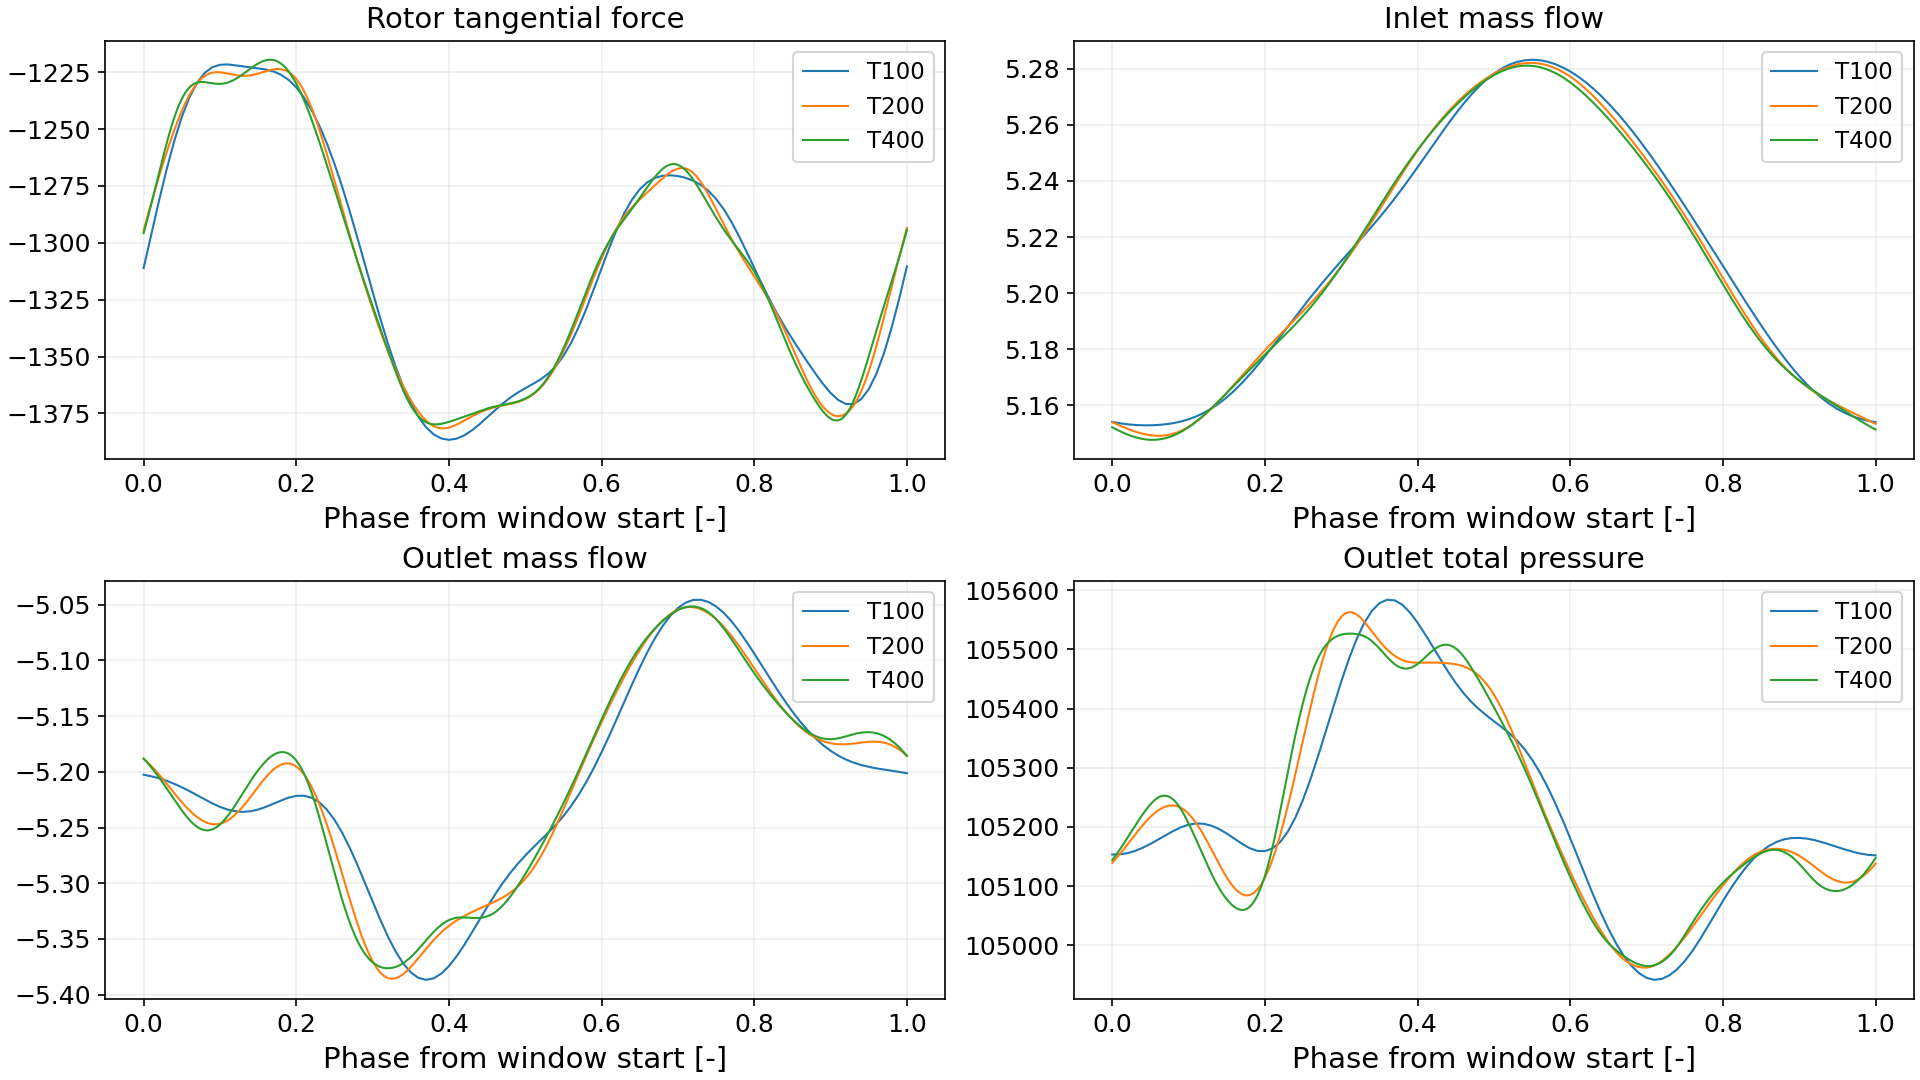
\includegraphics[width=\linewidth,height=0.42\textheight,keepaspectratio]{images/timestep_phase_profiles.png}
\caption{T100, T200 and T400 monitor profiles on the same fixed adapted mesh. Remaining amplitude differences preclude a general timestep-independence claim.}
\label{fig:9}
\end{figure}
\par
\subsection{Three-mesh sensitivity verified from accepted native monitors}
Three-mesh sensitivity was evaluated directly from the accepted native monitor segments. Source hashes, complete step sequences, physical clocks, three-cycle means and cycle amplitudes were checked against the saved analyses. All meshes used T/400 and 30 inner iterations. M1 and M3 were assessed over cycles 33-35, and M2 over cycles 38-40. The windows have equal duration and matching rotor phase, although residual transient differences can remain. The resulting differences therefore describe finite-window mesh sensitivity rather than an isolated spatial discretization error.\par

\begin{equation}
\delta_{\overline q}=100\frac{|\overline q_c-\overline q_f|}{|\overline q_f|},\qquad
\delta_{\overline A}=100\frac{|\overline A_c-\overline A_f|}{\overline A_f}.
\end{equation}
\par
\begin{table}[!htbp]
\centering
\caption{Direct grid-sensitivity audit. Relative differences use the finer-mesh output as denominator; the phase RMS denominator is its mean cycle peak-to-peak amplitude.}
\label{tab:14}
\small\renewcommand{\arraystretch}{1.16}
\begin{tabularx}{\linewidth}{@{}>{\raggedright\arraybackslash}X >{\raggedright\arraybackslash}X >{\raggedright\arraybackslash}X >{\raggedright\arraybackslash}X >{\raggedright\arraybackslash}X@{}}
\toprule
\textbf{Quantity} & \textbf{M1-M2 mean [\%]} & \textbf{M2-M3 mean [\%]} & \textbf{M2-M3 amplitude [\%]} & \textbf{M2-M3 phase RMS / amplitude [\%]} \\
\midrule
Rotor tangential force & 0.1861 & 0.1338 & 6.4156 & 3.5075 \\
Inlet mass flow & 0.1192 & 0.0282 & 7.1206 & 5.6922 \\
Outlet mass flow & 0.2176 & 0.1377 & 7.5185 & 4.0220 \\
Outlet total pressure & 0.0027 & 0.0439 & 5.8633 & 8.0058 \\
\bottomrule
\end{tabularx}
\end{table}
\par
All four M2-M3 mean differences are below 0.15\%: force 0.1338\%, inlet flow 0.0282\%, outlet flow 0.1377\% and total pressure 0.0439\%. This supports the limited statement that these means are weakly sensitive to the last tested refinement. The amplitude differences remain 6.4156\%, 7.1206\%, 7.5185\% and 5.8633\%, respectively. Phase-profile RMS differences reach 8.0058\% of the finer-grid amplitude. The oscillating part of the solution is therefore still mesh sensitive.\par

\par
\begin{figure}[!htbp]
\centering
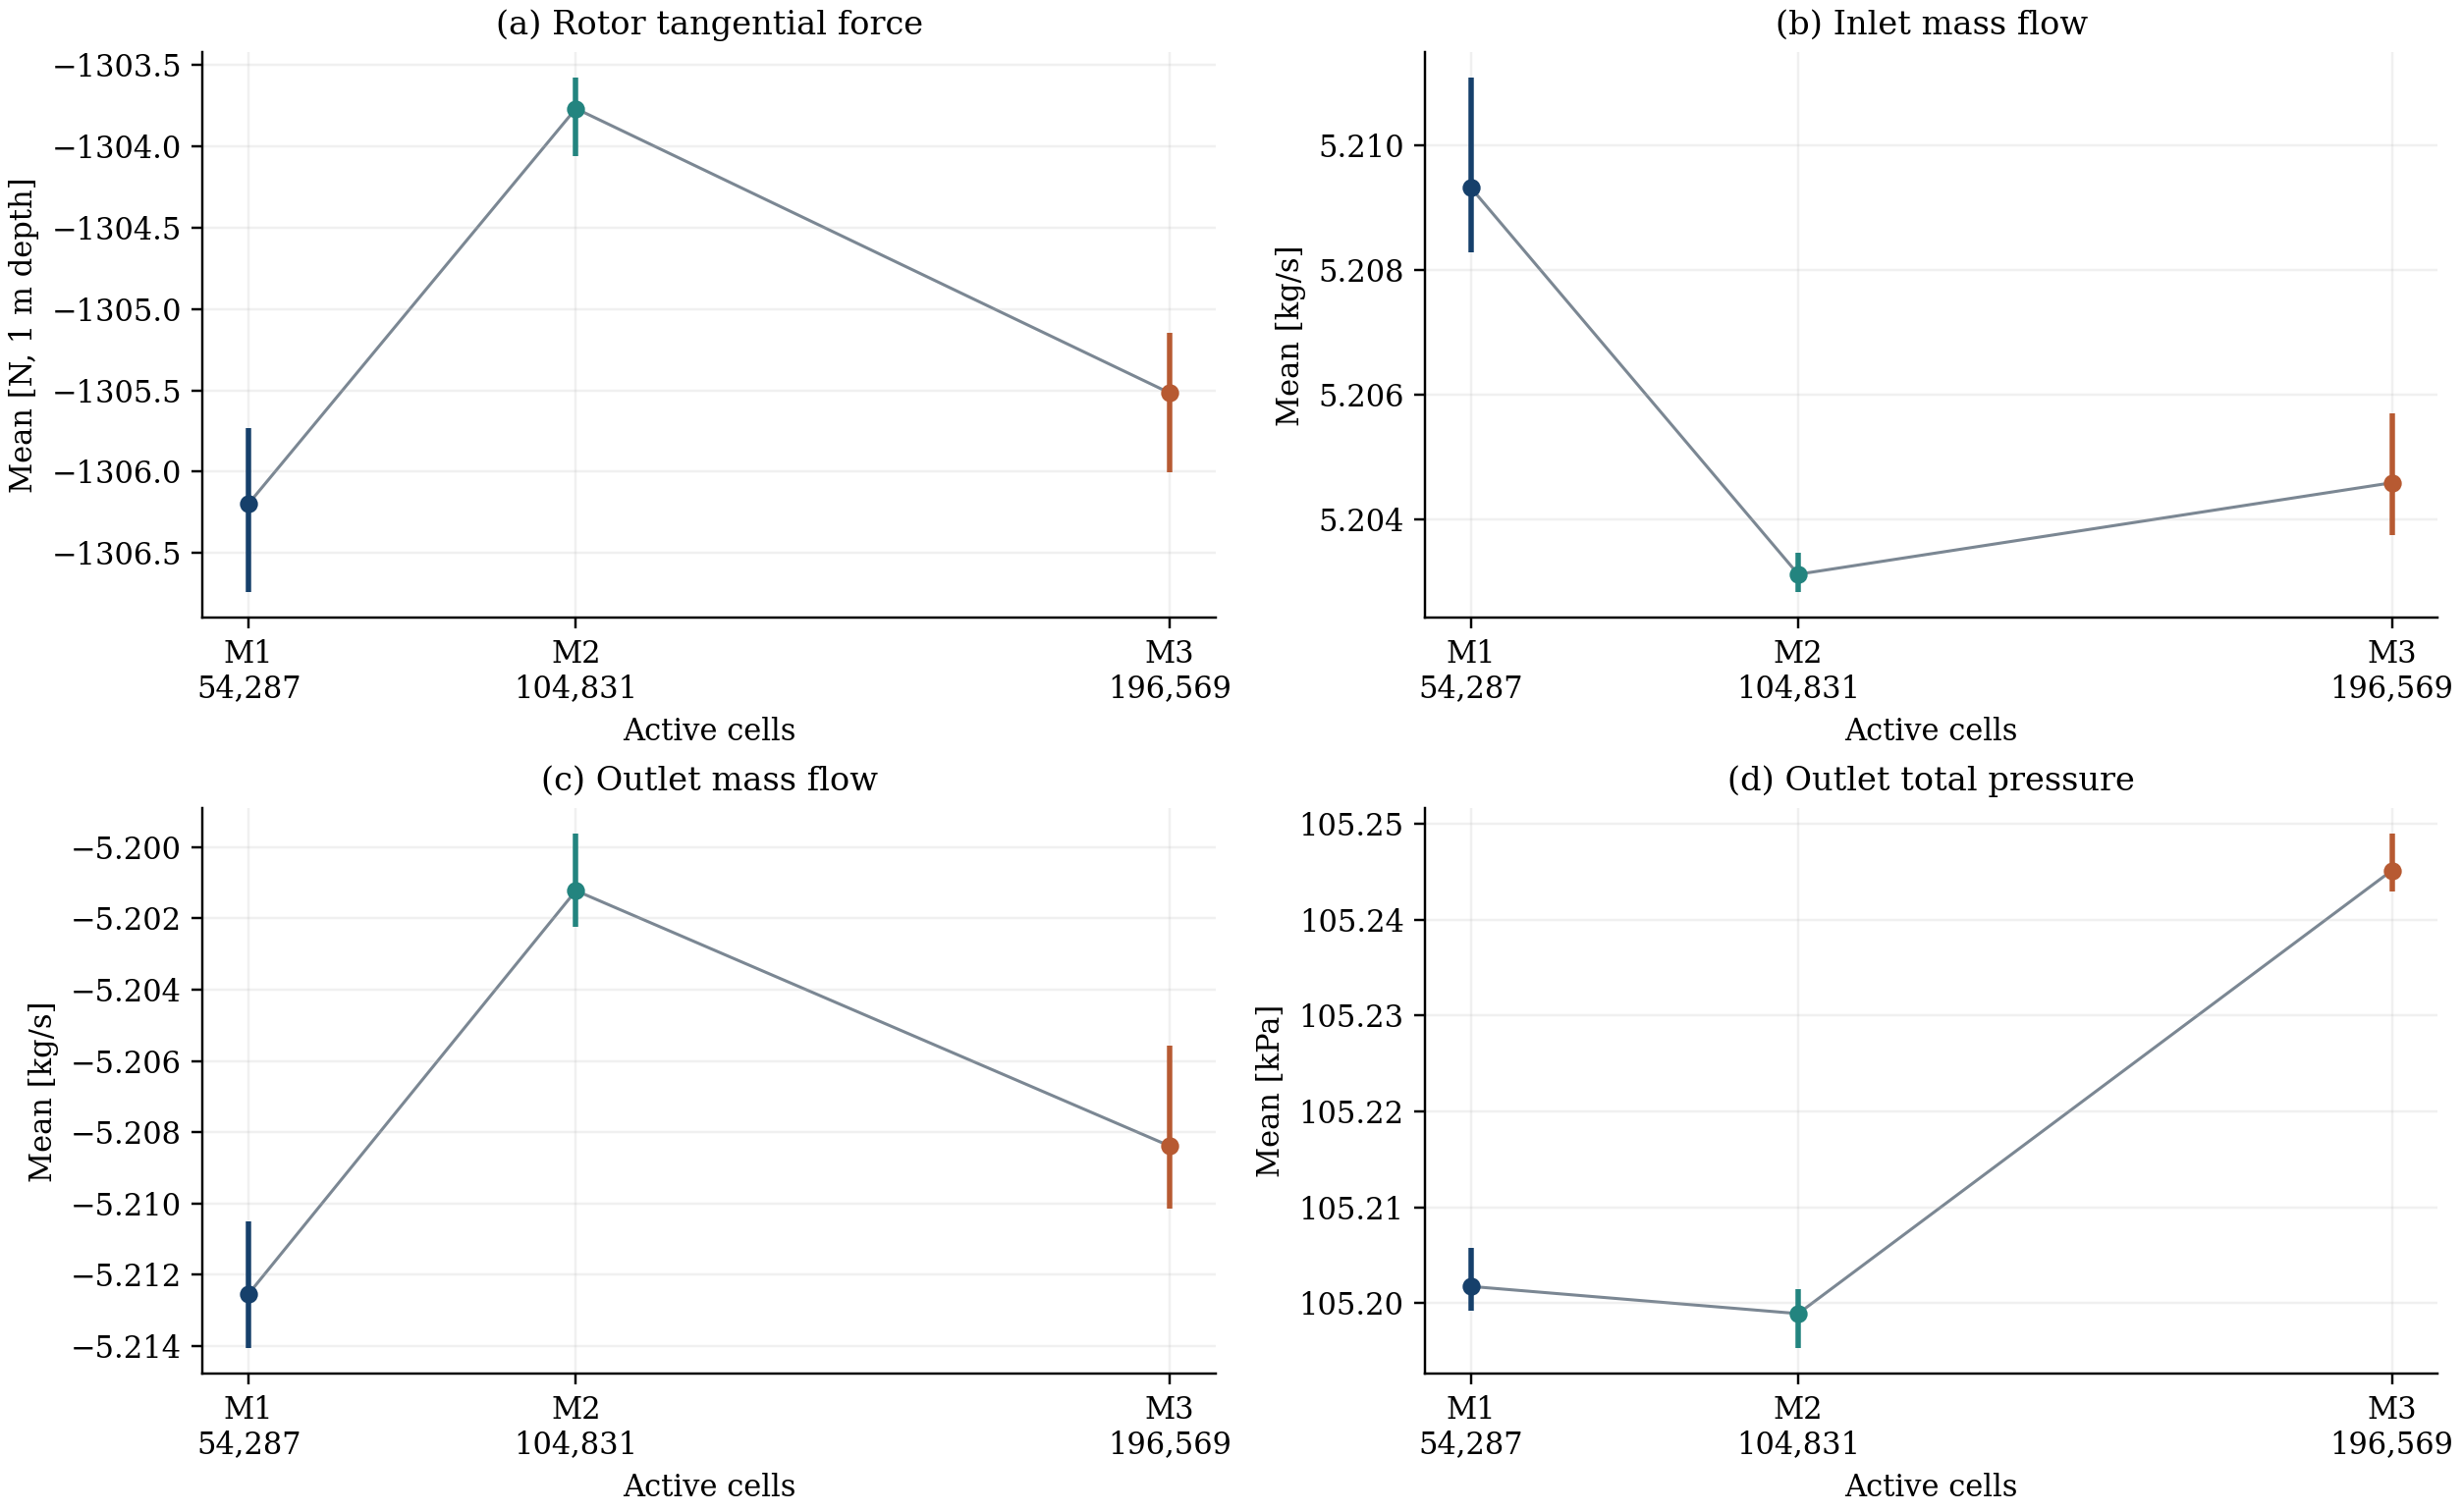
\includegraphics[width=\linewidth,height=0.42\textheight,keepaspectratio]{images/grid_cycle_means.png}
\caption{Systematic-mesh cycle means recalculated from native monitors. Vertical ranges span the three observed cycle means; they are not confidence intervals or grid-error bars. Small vertical differences should not be confused with a monotonic asymptotic trend.}
\label{fig:10}
\end{figure}
\par
\par
\begin{figure}[!htbp]
\centering
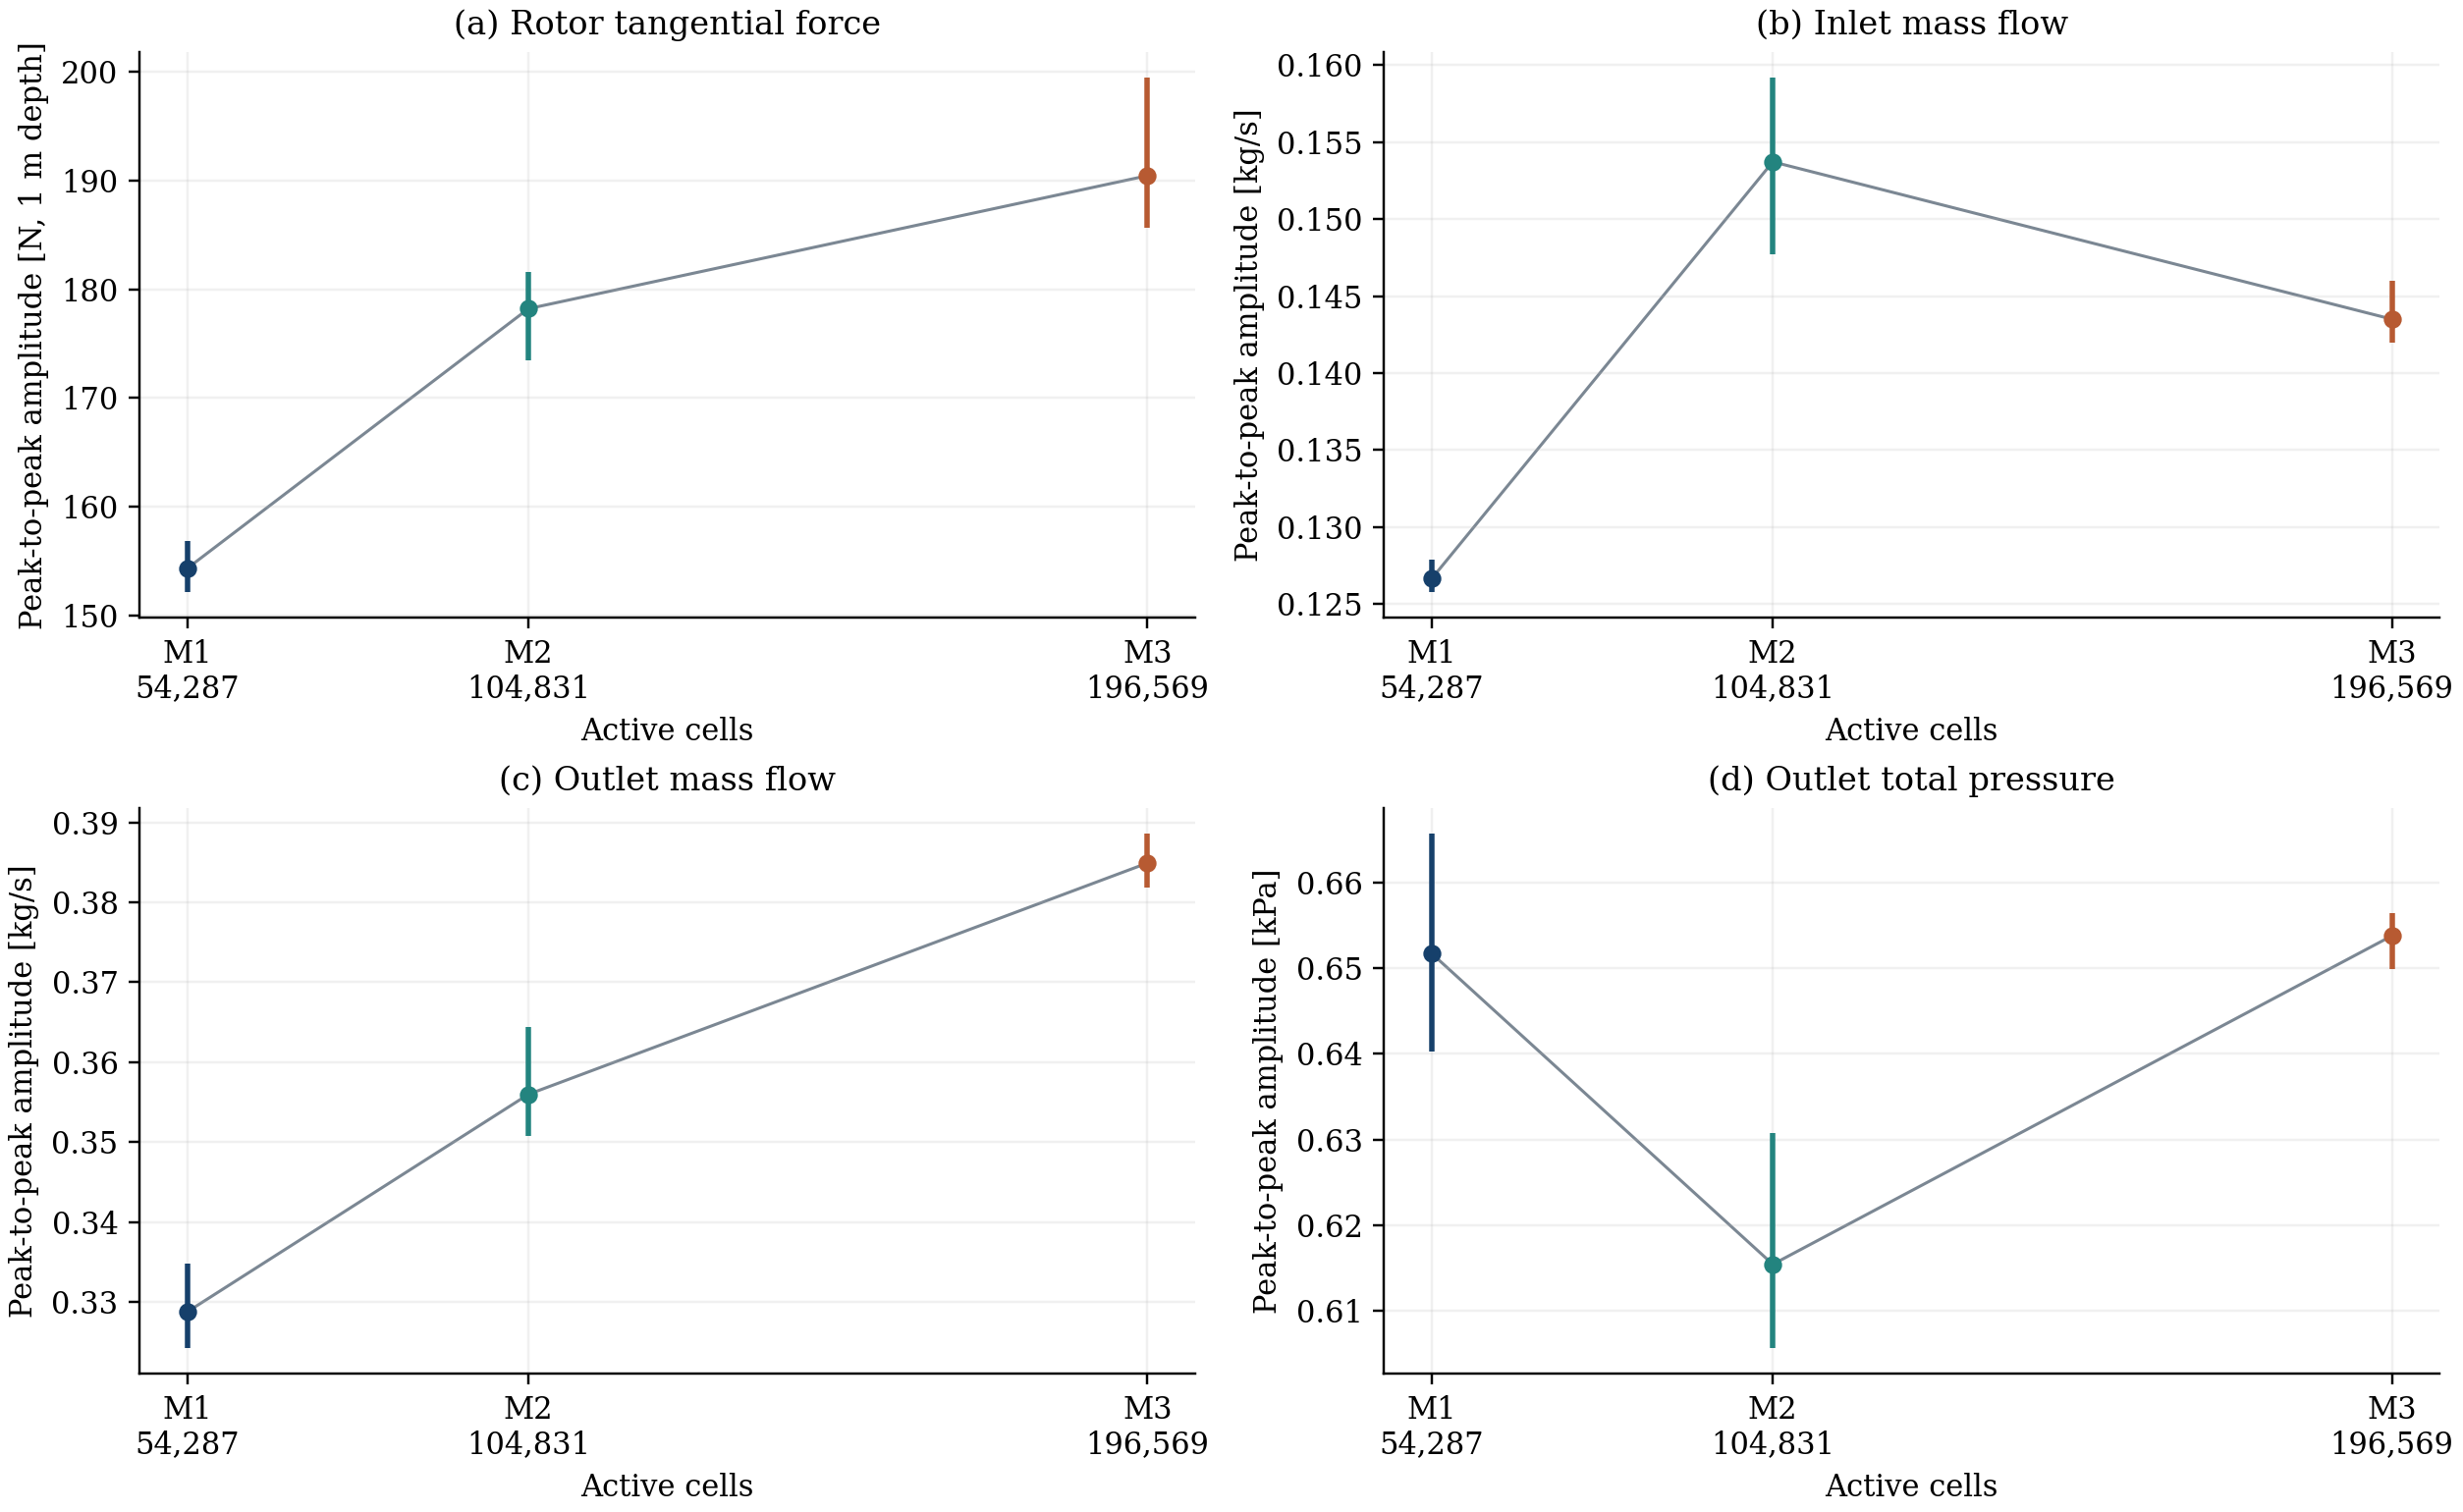
\includegraphics[width=\linewidth,height=0.42\textheight,keepaspectratio]{images/grid_cycle_amplitudes.png}
\caption{Systematic-mesh peak-to-peak amplitudes. Points are the average of three cycle amplitudes; vertical ranges show the observed cycle variation. Force and outlet-flow amplitudes continue to increase with refinement.}
\label{fig:11}
\end{figure}
\par
\par
\begin{figure}[!htbp]
\centering
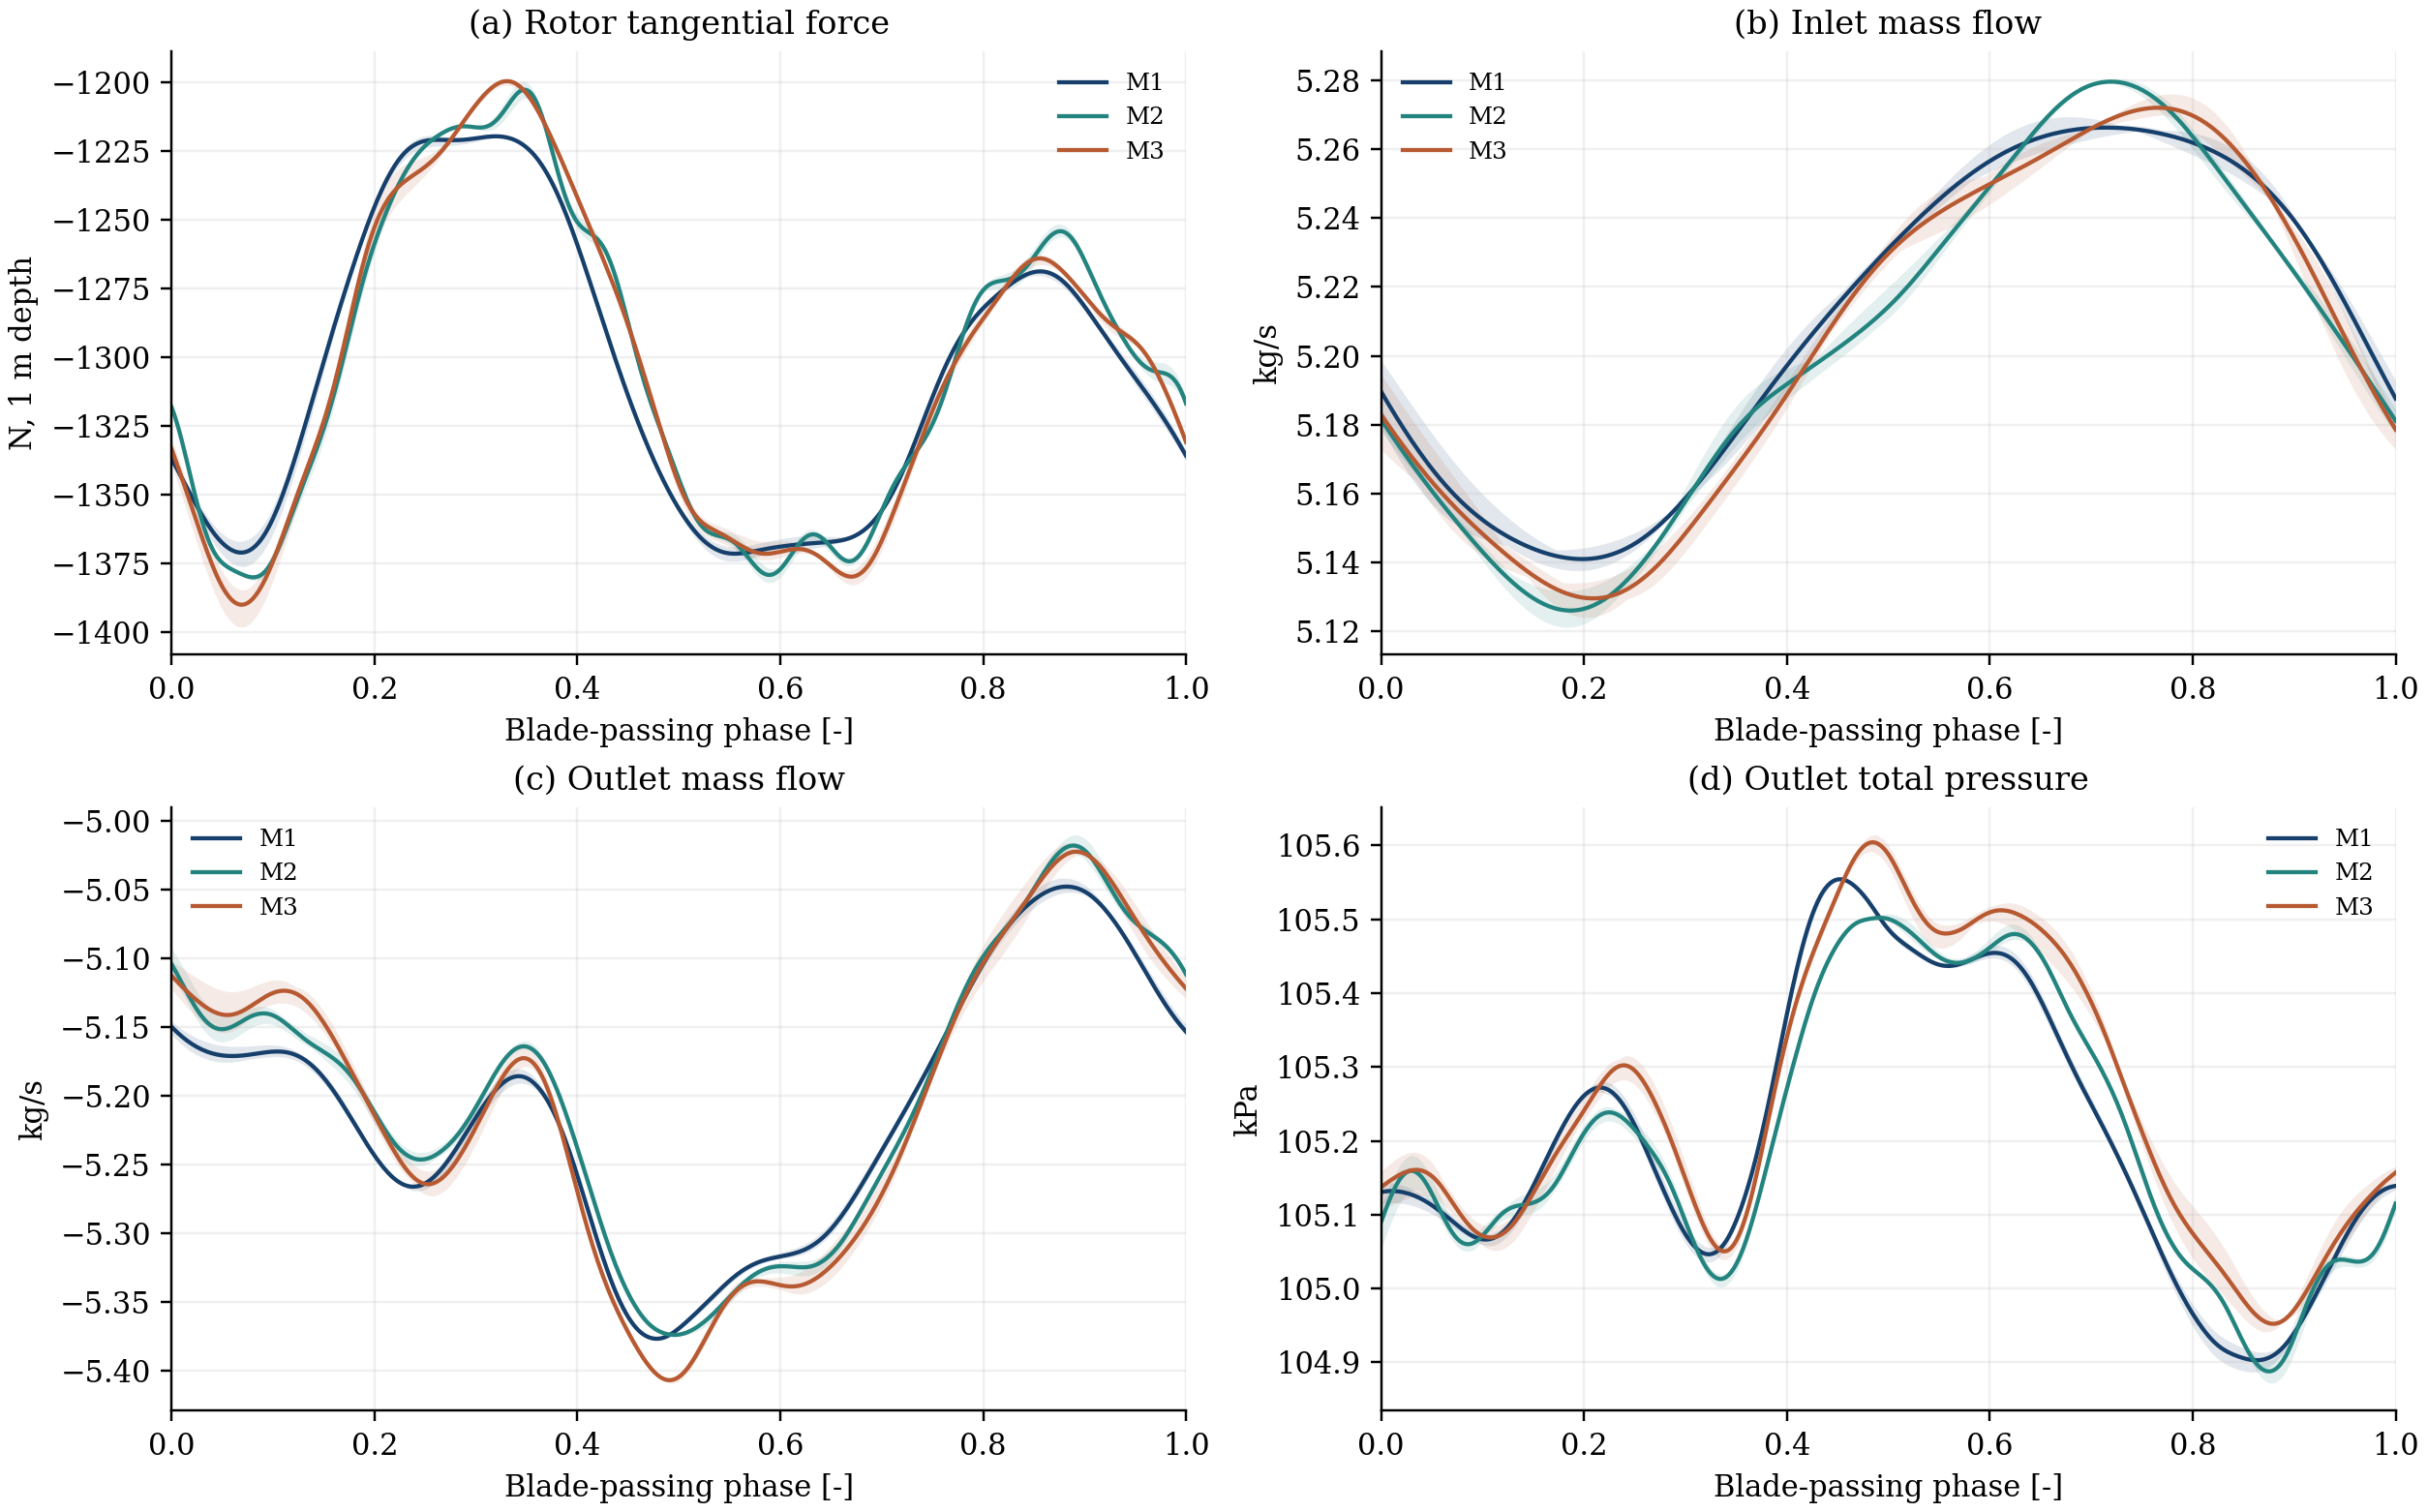
\includegraphics[width=\linewidth,height=0.42\textheight,keepaspectratio]{images/grid_phase_profiles.png}
\caption{Three-mesh profiles at common blade-passing phase. Lines are the three-cycle phase means; shaded bands span the observed cycles. M2 was sampled five periods later than M1/M3, so residual settling can contaminate mesh differences.}
\label{fig:12}
\end{figure}
\par
\subsection{Asymptotic range and GCI assessment}
All four cycle-mean sequences reverse direction between M1-M2 and M2-M3. Total-pressure mean changes increase from 0.0027\% to 0.0439\% rather than contracting. Force and outlet-flow amplitudes increase monotonically, but their changes do not establish a common asymptotic error model. Inlet and total-pressure amplitudes are nonmonotonic. A small last-pair mean difference alone does not determine the continuum limit or a general error band.\par

Indicative two-dimensional cell-count refinement ratios are 1.38962 for M1-M2 and 1.36934 for M2-M3, using h proportional to the inverse square root of cell count. They are close to the nominal refinement, but do not prove a single h scale for this anisotropic inflation family. Together with unresolved cycle and timestep sensitivity, the present data do not justify assigning an observed convergence order or GCI. NASA guidance treats assessment of the asymptotic range and the separation of error sources as part of solution verification; the applicable sources are listed in the references.\par

The computed differences quantify sensitivity to refinement. General grid independence was not demonstrated. Mean outputs were weakly sensitive to the M2-M3 refinement within the assessed windows, whereas amplitudes and phase profiles retained appreciable differences. No observed convergence order or GCI was assigned.\par

\FloatBarrier
\section{Blade pressure, wall resolution and flow interpretation}
\subsection{Native wall-face data across the systematic meshes}
Final-cycle wall averages use five common phase samples, including the closing endpoint, at intervals T/4 on each mesh. The new comparison plots native wall-face values directly against axial position. Pressure and suction sides are not joined by an unverified interpolation, and no pointwise wall-error norm is claimed. The pressure distributions almost overlap at the plotted scale; refinement visibly reduces y+ while all sampled maxima remain below one.\par

\par
\begin{figure}[!htbp]
\centering
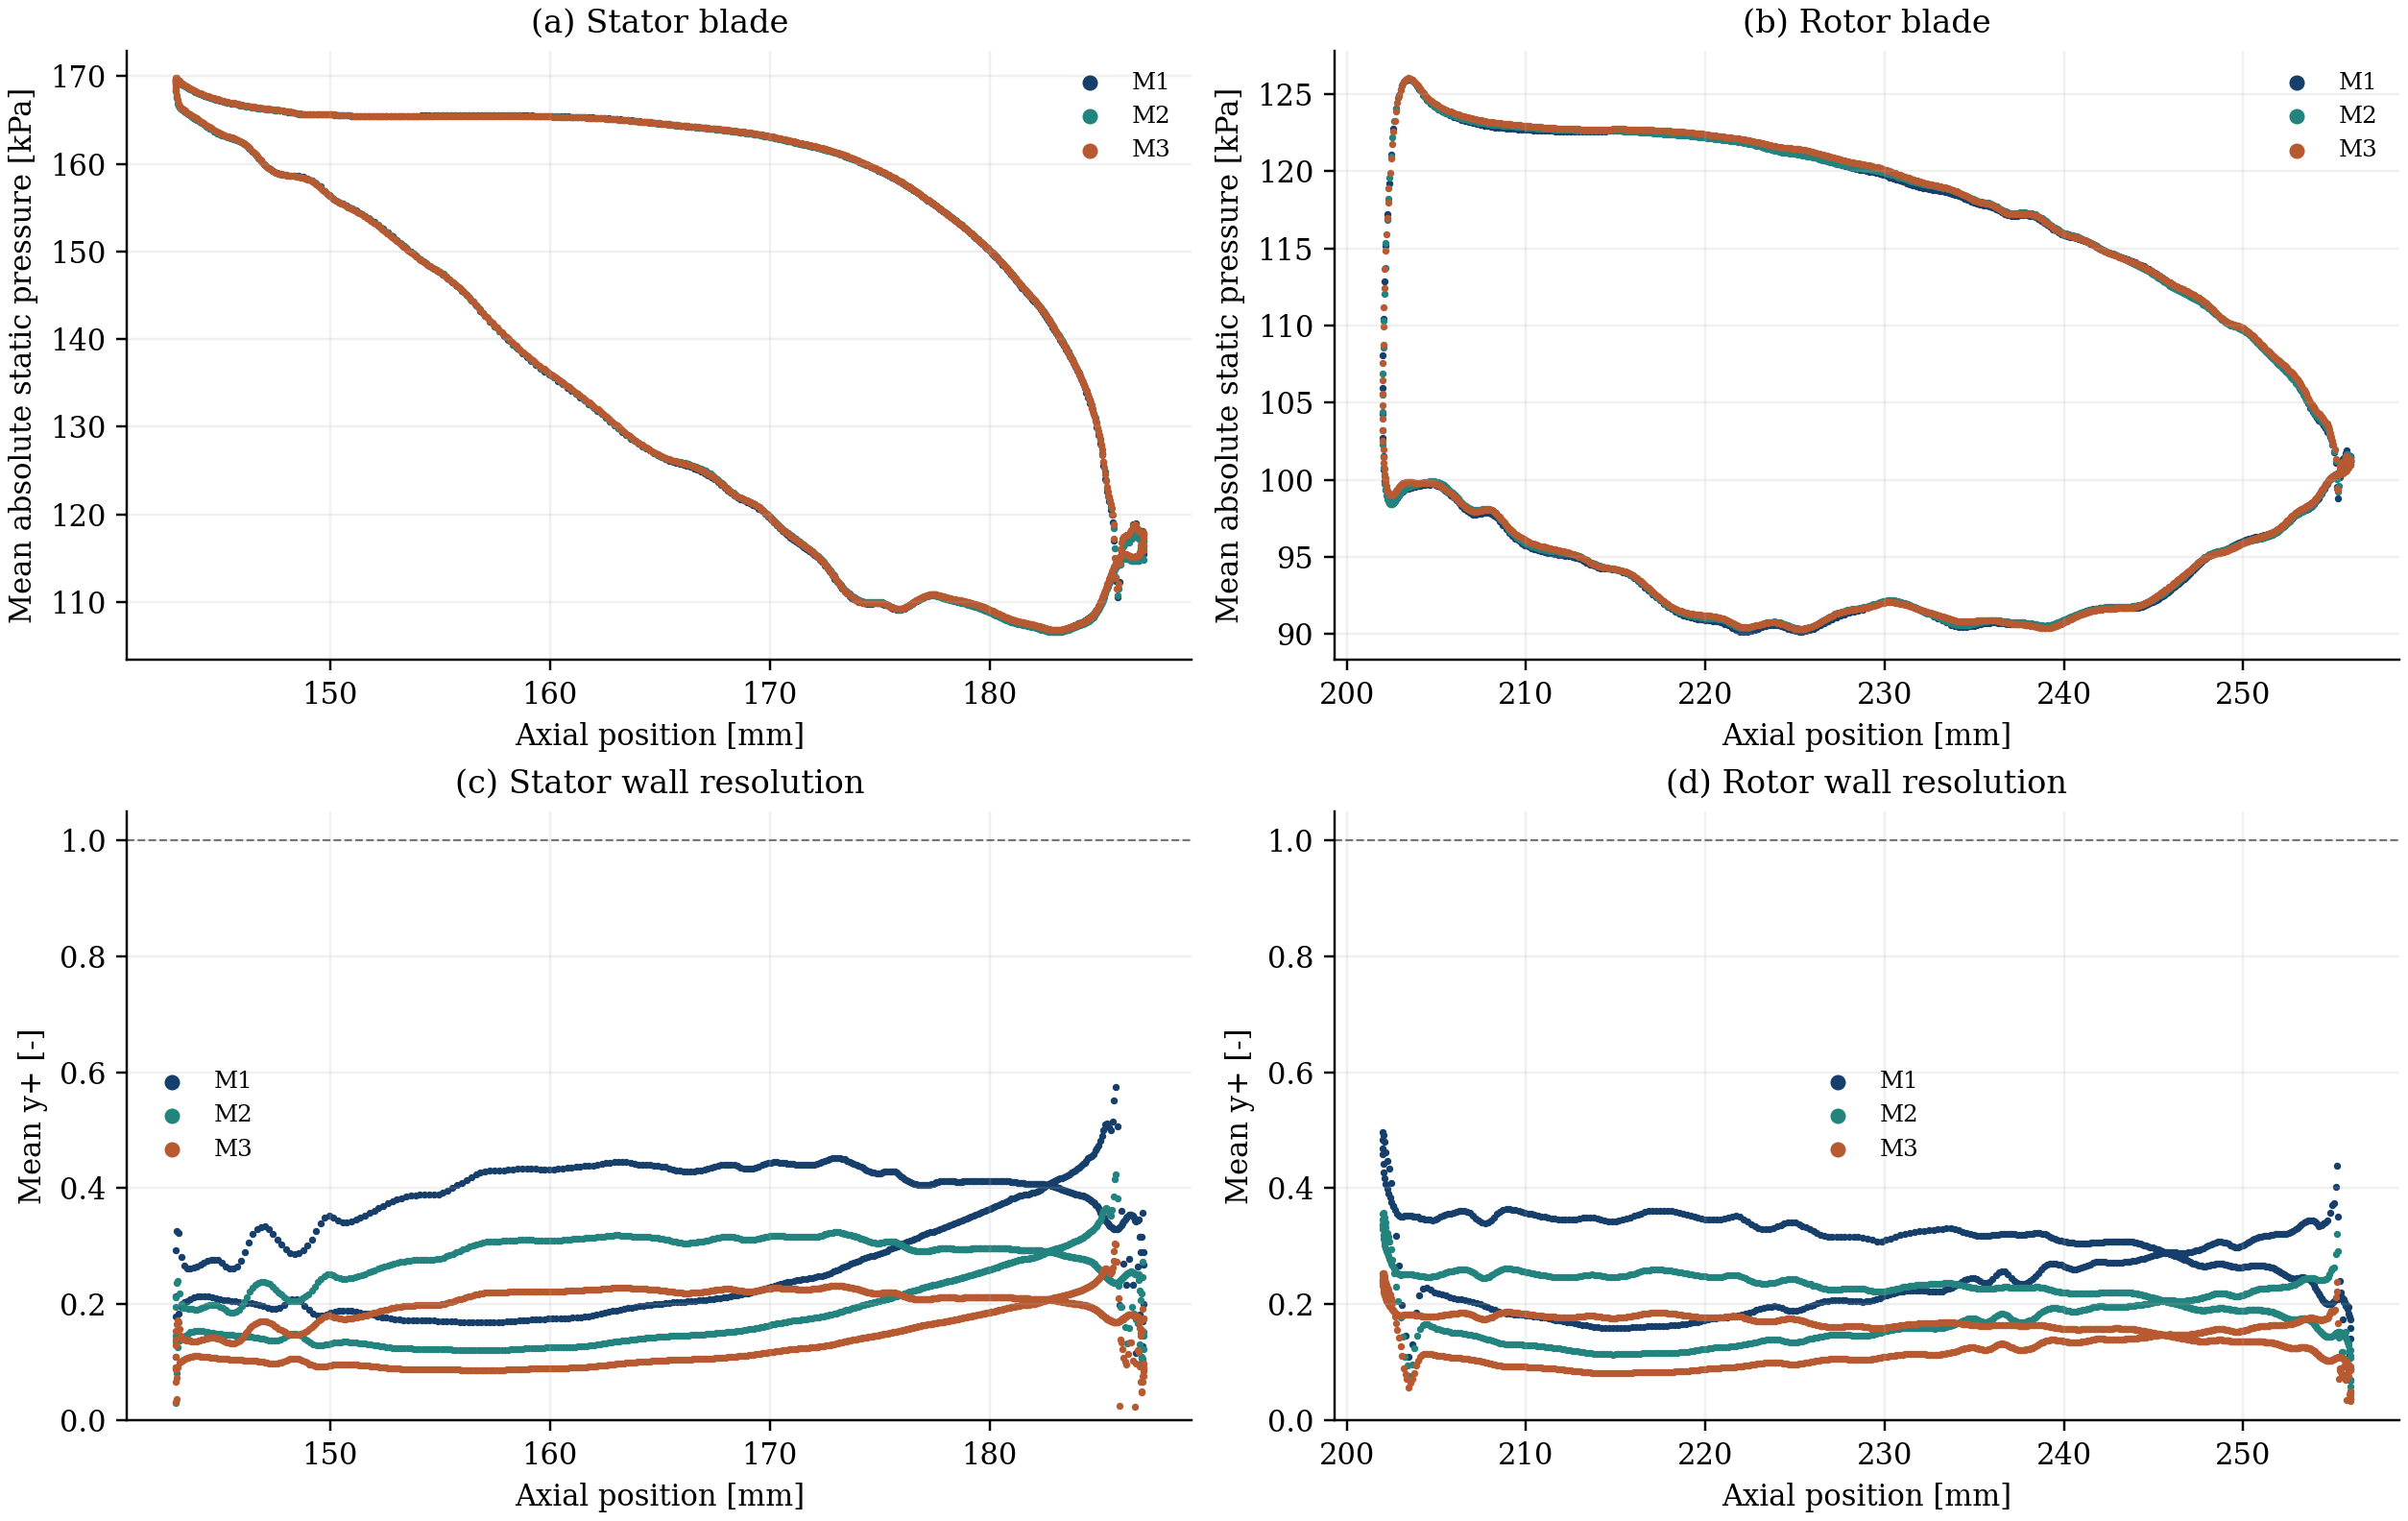
\includegraphics[width=\linewidth,height=0.42\textheight,keepaspectratio]{images/grid_blade_pressure_yplus.png}
\caption{Cycle-mean absolute static pressure and y+ on both blades for M1/M2/M3. Five phase samples per final cycle are used. These profiles show finite-window sensitivity; sampled y+ does not bound unsaved phases.}
\label{fig:13}
\end{figure}
\par
For M3, sampled maximum y+ is 0.30818 on the stator and 0.26818 on the rotor. The three-cycle mean tangential force is -1305.516 N, mean inlet mass flow 5.204588 kg/s, outlet mass flow -5.208388 kg/s and mass-flow-weighted outlet total pressure 105245.147 Pa. These remain diagnostic finite-window values, not certified periodic turbine performance.\par

\subsection{Reference-frame and performance limits}
Native Mach is absolute and was checked against velocity magnitude divided by sound speed. Blade-wall velocity confirms that rotor mesh motion is applied once. Static pressure is absolute because operating pressure is zero. Total-pressure change across the moving row includes work transfer; it is not presented as a standalone entropy or loss measure. No experimental validation or model-form uncertainty estimate is available.\par

\FloatBarrier
\section{Visualisation and animation products}
The fixed-adapted-mesh T400 dataset provides synchronized absolute-Mach and absolute-static-pressure animations with fixed legends and verified periodic translations. A separate fine-mesh M3 movie represents the accepted absolute-Mach interval from 5T to 35T. Mach-only acquisition was used for the fine-mesh transient to limit graphics overhead. These visualisation products correspond to different datasets and were interpreted separately.\par

\par
\begin{table}[!htbp]
\centering
\caption{Verified M3 animation configuration and available interval}
\label{tab:15}
\small\renewcommand{\arraystretch}{1.16}
\begin{tabularx}{\linewidth}{@{}>{\raggedright\arraybackslash}X >{\raggedright\arraybackslash}X@{}}
\toprule
\textbf{M3 animation parameter} & \textbf{Verified value} \\
\midrule
Physical interval [s] & 0.001487918925 - 0.010415432475 \\
Native steps / source PNGs & 2000-14000, every 10 steps; 1201 PNGs \\
Physical acquisition interval & 7.439594625e-6 s; 40 frame intervals per pitch period \\
Resolution / playback & 1920 x 1080; 25 FPS; 48.04 s \\
Mach legend & Fixed 0-1.2; values above 1.2 saturate the top colour and this is disclosed \\
Camera and repeat geometry & Fixed three-pitch crop; verified native periodic instances on both rows \\
Time annotation & Actual Fluent Solution time, 12 decimal places \\
Encoder & Offline H.264 from unchanged native Fluent PNGs; no CFD and no Fluent Playback \\
\bottomrule
\end{tabularx}
\end{table}
\par
Only frames associated with the accepted main solution were included in the M3 movie. The complete sequence from t=0 was not verified and is not reported as an available result. The verified interval is 5T-35T. The main 30T-35T continuation was checked independently against native time, mesh geometry, solver settings, report values and BDF2 histories before advancing.\par

The final MP4 was decoded for beginning, quarter-phase motion, middle and end samples. Blade rows, fixed legend size, camera, physical clock and annotation were visually checked. Image hashes and dimensions were checked for all 1201 source frames. Sampling inspection does not establish temporal smoothness at every frame or periodic convergence. Camera cropping naturally shows partial blades at its upper and lower boundaries as the row translates. Playback FPS is distinct from physical acquisition rate.\par

\par
\begin{figure}[!htbp]
\centering
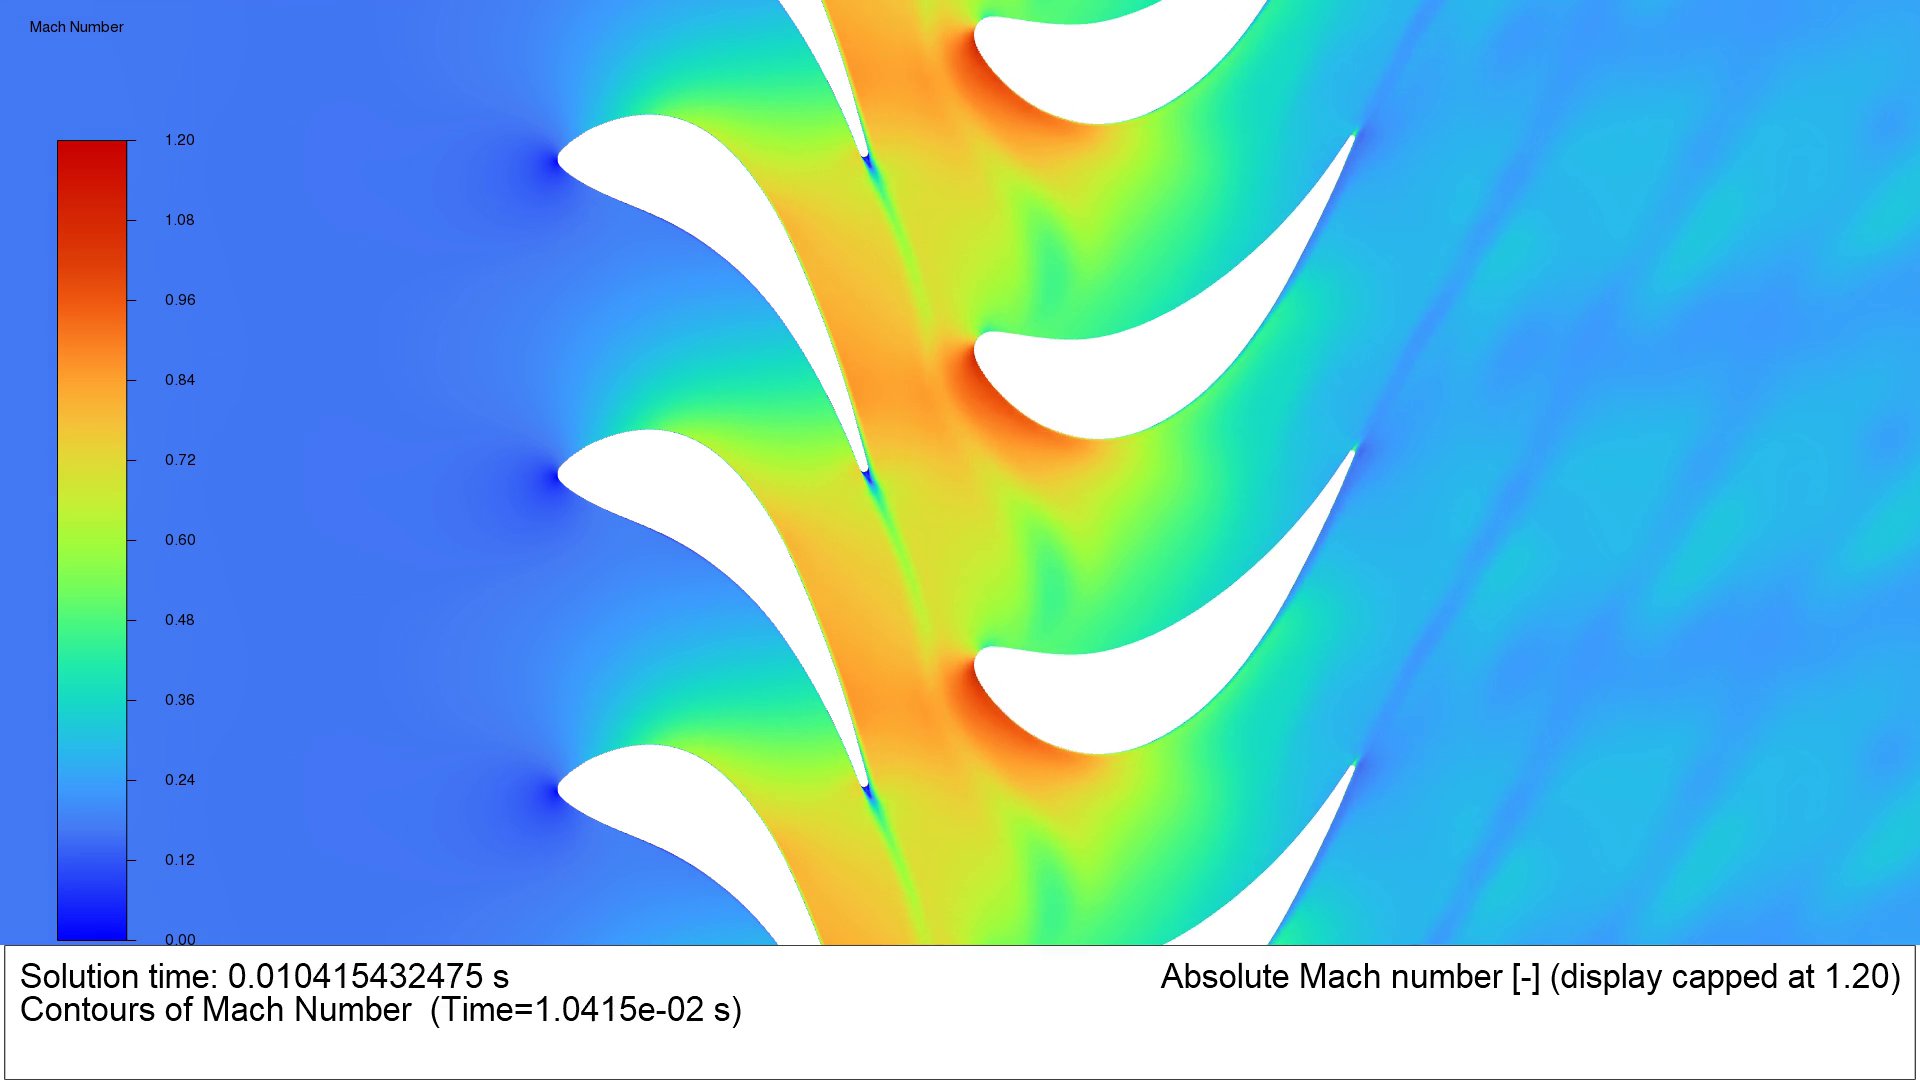
\includegraphics[width=\linewidth,height=0.42\textheight,keepaspectratio]{images/m3_mach_35_periods.png}
\caption{Fine-mesh absolute Mach field at 35T, with three visible pitches and a fixed 0-1.2 display cap. Upper-colour saturation is explicitly disclosed. The annotation uses the actual physical Fluent clock.}
\label{fig:14}
\end{figure}
\par
\par
\begin{figure}[!htbp]
\centering
\begin{subfigure}[t]{0.48\linewidth}\centering
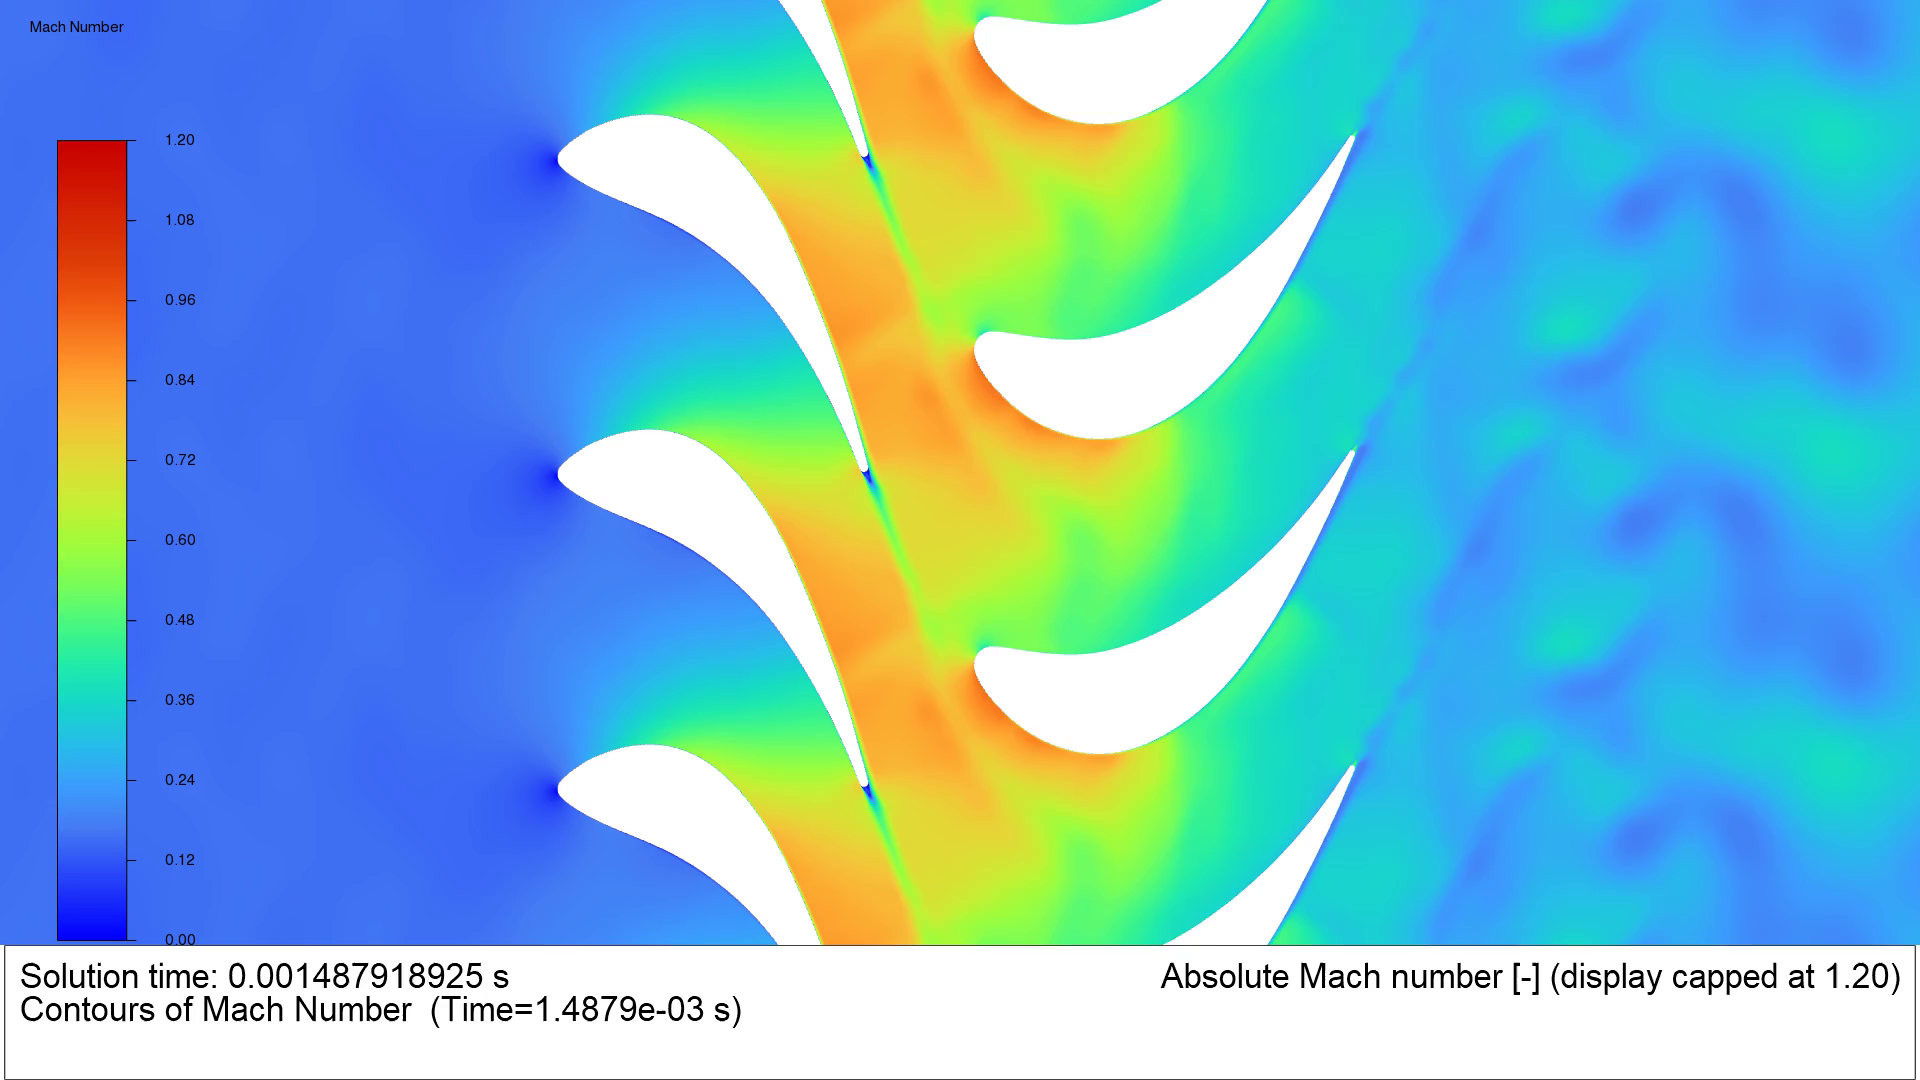
\includegraphics[width=\linewidth,height=0.25\textheight,keepaspectratio]{images/m3_mach_5_periods.png}
\caption{M3 at 5T}
\end{subfigure}
\hfill
\begin{subfigure}[t]{0.48\linewidth}\centering
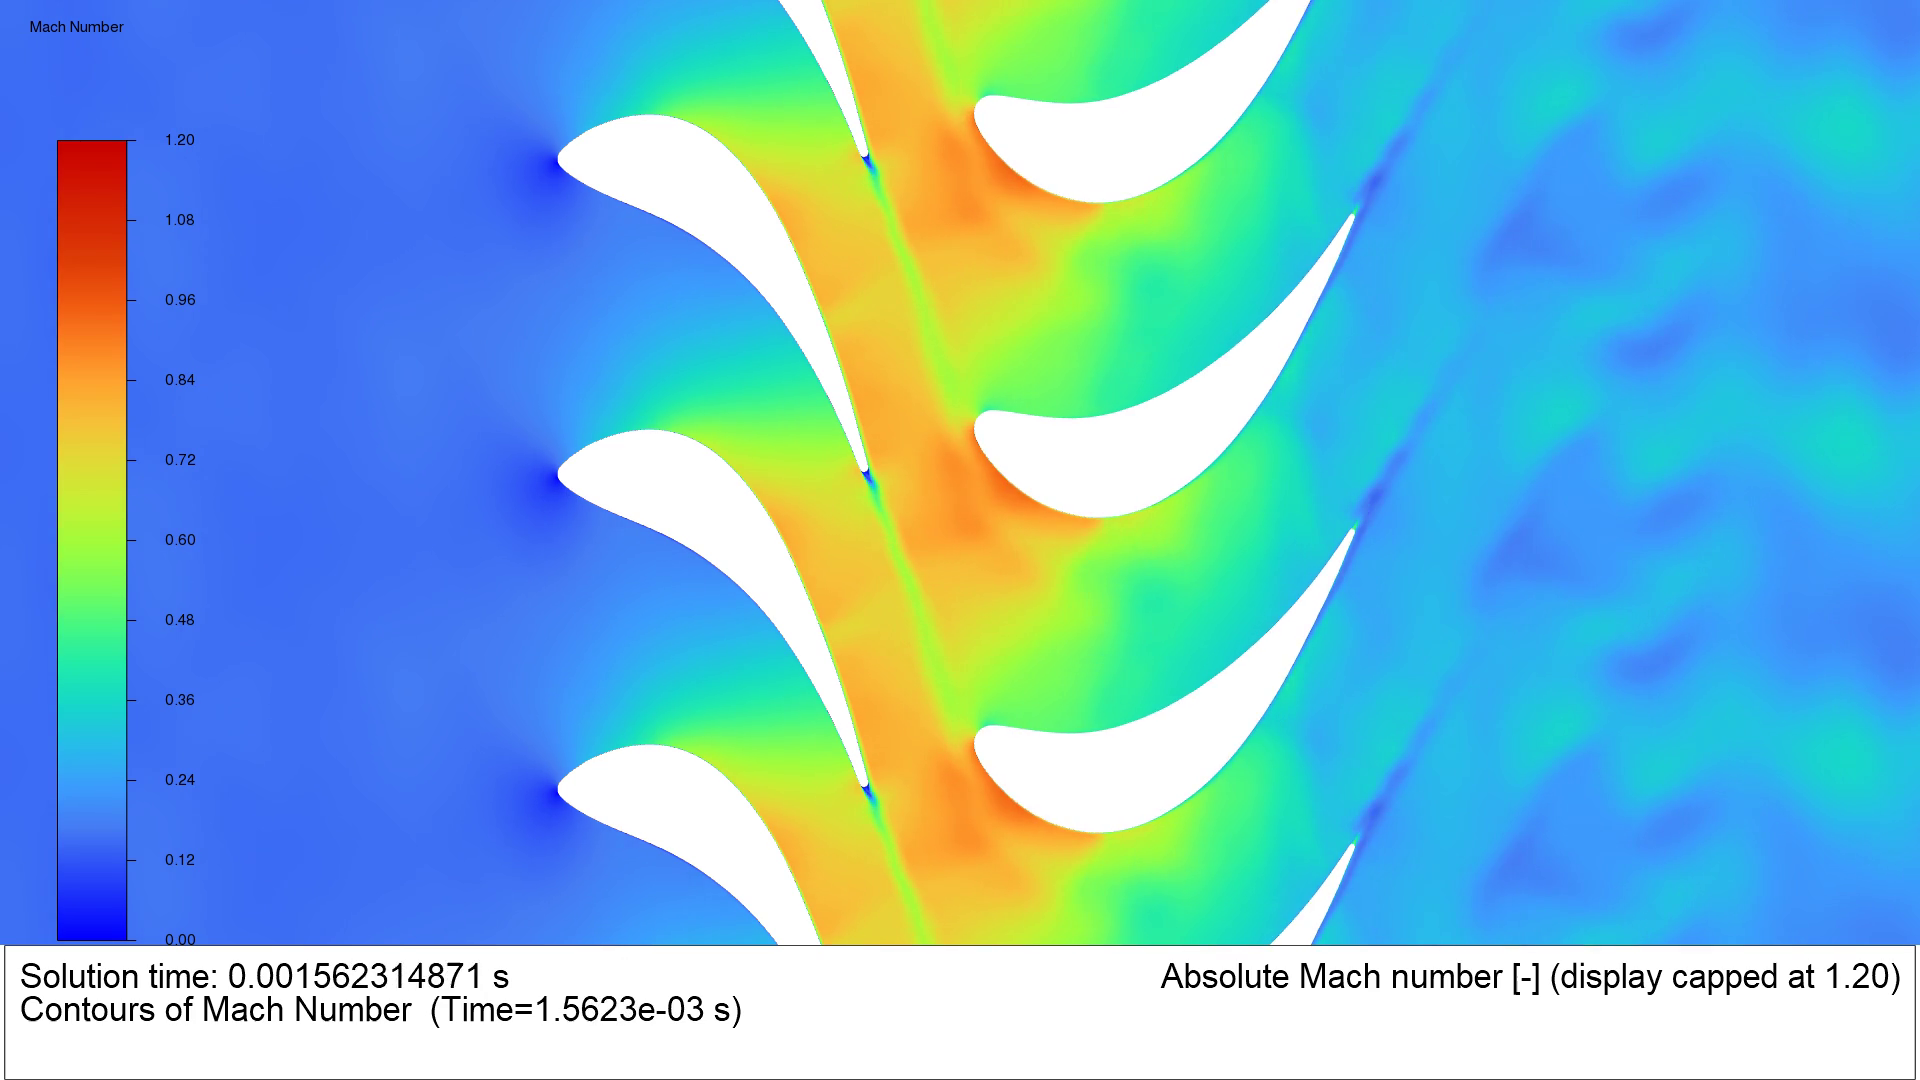
\includegraphics[width=\linewidth,height=0.25\textheight,keepaspectratio]{images/m3_mach_5p25_periods.png}
\caption{M3 at 5.25T}
\end{subfigure}
\par\vspace{0.65em}
\caption{Quarter-period rotor displacement in decoded native-PNG movie frames. Camera, periodic crop and colour-bar geometry are unchanged. This visual check is distinct from the unresolved periodicity of the flow.}
\label{fig:15}
\end{figure}
\par
\FloatBarrier
\section{Discussion and limits of the present results}
\par
\begin{table}[!htbp]
\centering
\caption{Final interpretation by verification topic}
\label{tab:16}
\small\renewcommand{\arraystretch}{1.16}
\begin{tabularx}{\linewidth}{@{}>{\raggedright\arraybackslash}X >{\raggedright\arraybackslash}X@{}}
\toprule
\textbf{Topic} & \textbf{Final conclusion} \\
\midrule
Historical baseline & Coherent reopened reference; AMR history distinguished from currently disabled AMR \\
Restart and automation & Verified smoke tests and strict native continuation; historical failures retained separately \\
Iteration sensitivity & 30/60 comparison supports 30 on the adapted mesh; not a separate proof for M3 \\
Timestep sensitivity & T200/T400 amplitude criterion not met; timestep independence unconfirmed \\
M1 original-position Hybrid & 35 periods; recorded operational settling checks passed \\
M2 original-position Hybrid & 40 periods; inlet-amplitude recurrence still fails the three-cycle limit \\
M3 original-position Hybrid & 35 periods; force-amplitude recurrence still fails one cycle pair \\
Spatial convergence / GCI & Not established; no observed order or error bar assigned \\
M3 video & Verified available 5T-35T transient interval; complete t=0 sequence unverified \\
Validation & No experimental validation and no certified turbine performance claim \\
Simulated duration & M1: 35 periods; M2: 40 periods; M3: 35 periods; finite-window limitations retained \\
\bottomrule
\end{tabularx}
\end{table}
\par
Residual amplitude evolution can remain after cycle means and mass conservation appear stable. The available data do not uniquely separate transient evolution, sampling sensitivity and numerical error. Mesh quality and sampled wall resolution provide useful numerical checks, but do not establish spatial independence or physical accuracy.\par

The four mean quantities differ by at most 0.138\% between M2 and M3, while amplitude changes remain above 5.8\%. These observations indicate different sensitivities for different quantities of interest. The nonmonotonic three-mesh means do not support a formal convergence-order estimate or a GCI error bar.\par

\FloatBarrier
\section{Conclusions}
The historical baseline and Workbench dependencies are preserved, native restarts and original-position Hybrid starts are traceable, and the systematic family has verified positive-volume mesh-quality and sampled wall-resolution data. The workflow produced accepted monitor histories, conservation audits, English figures and an explicitly scoped Mach movie.\par

The three-grid assessment was based on saved native data. Last-pair means were weakly sensitive to refinement, while amplitudes and phase waveforms retained appreciable mesh sensitivity. Periodic settling on M2/M3 and temporal independence remained unresolved. The reported durations were 35 periods for M1, 40 for M2 and 35 for M3; general spatial independence and an asymptotic GCI were not established.\par

\FloatBarrier
\appendix
\section{Data availability and reproducibility}
The numerical dataset comprises the historical reference pair, the systematic mesh files, coherent final case/data pairs, accepted native monitor segments, sampled phase fields, wall-face exports and numerical verification tables. Solver settings, timestep, internal iteration count, mesh size, reference depth and physical-time intervals are recorded alongside each result. Intermediate checkpoints and superseded development outputs are retained separately in the private technical archive.\par
The repository separates flat Python modules in \path{workflow/}, configuration in \path{config/}, geometry and source attribution in \path{geometry/}, and selected numerical tables, figures and animations in \path{results/}. The report source and images form a self-contained LaTeX project in \path{docs/report/}. Large native input files in \path{inputs/} and solver output directories in \path{runs/} are local resources excluded from normal Git history. Run identifiers and SHA256 manifests associate the publication figures and tables with their numerical sources. ANSYS software and the Python runtime are not redistributed.\par
\FloatBarrier
\begin{thebibliography}{9}
\addcontentsline{toc}{section}{References}
\bibitem{su2} S. Vitale, Delft University of Technology. SU2 TestCases: axial\_stage\_2D, configuration dated 28 February 2017, file version 8.5.0 Harrier. \url{https://github.com/su2code/TestCases/tree/master/turbomachinery/axial_stage_2D}. The original source attribution and LGPL 2.1 licence text are retained with the reference material.
\bibitem{fluent} ANSYS. Fluent User's Guide, Release 2024 R2. Mesh modification and native mesh-to-mesh interpolation. \url{https://ansyshelp.ansys.com/public/Views/Secured/corp/v242/en/flu_ug/flu_ug_GridModify.html}; \url{https://ansyshelp.ansys.com/public/Views/Secured/corp/v242/en/flu_ug/flu_ug_Grid_to_Grid.html}.
\bibitem{pyfluent} PyAnsys. Official PyFluent documentation and version-specific generated interfaces for Fluent 2024 R2. \url{https://fluent.docs.pyansys.com/}.
\bibitem{nasa_grid} NASA NPARC Alliance. Examining Spatial (Grid) Convergence. \url{https://www.grc.nasa.gov/www/wind/valid/tutorial/spatconv.html}.
\bibitem{nasa_verify} NASA NPARC Alliance. Verification Assessment. \url{https://www.grc.nasa.gov/www/wind/valid/tutorial/verassess.html}.
\end{thebibliography}
\end{document}
